% mnras_template.tex 

\documentclass[fleqn,usenatbib]{mnras}

% Use Times font
\usepackage{newtxtext,newtxmath}

% Standard packages
\usepackage[T1]{fontenc}
\usepackage{graphicx}
\usepackage{amsmath}
\usepackage{booktabs}
\usepackage{hyperref}
\usepackage{float}
\usepackage{dblfloatfix}
\usepackage{subcaption}
\usepackage{xcolor}
\usepackage{placeins}  % For \FloatBarrier
\newcommand{\ar}[1]{\textcolor{blue}{#1}}
\newcommand{\je}[1]{\textcolor{orange}{#1}}

% Title of the paper
\title[Optimized Clustering for CMB Component Separation]{A novel approach to optimize clustering of parametric map-based component separation for upcoming CMB polarization satellites}

% Author list
\author[W. Kabalan et al.]{
Wassim Kabalan$^{1}$\thanks{Contact: \href{mailto:wassim@apc.in2p3.fr}{wassim@apc.in2p3.fr}}, 
Arianna Rizzieri,
Wuhyun Sohn$^{1}$,
Benjamin Beringue$^{1}$,
Artem Basyrov$^{1}$,
\newauthor
Pierre Chanial$^{1}$,
Alexandre Boucaud$^{1}$,
Josquin Errard$^{1}$\thanks{Contact: \href{mailto:josquin@apc.in2p3.fr}{josquin@apc.in2p3.fr}}
\\
$^{1}$Université Paris Cité, CNRS, Astroparticule et Cosmologie, F-75013 Paris, France
}
%Comment

% Publication details (filled by publisher later)
\date{Accepted XXX. Received YYY; in original form ZZZ}
\pubyear{\the\year{}}

% Don't change these lines
\begin{document}
\label{firstpage}
\pagerange{\pageref{firstpage}--\pageref{lastpage}}
\maketitle

\begin{abstract}
We present a novel \texttt{JAX}-powered parametric component separation approach that optimizes the degrees of freedom in the component separation parametrization, achieving minimum variance after foreground cleaning. This work is the first to incorporate an algorithm for optimizing the clustering of sky regions where the frequency scaling laws are assumed constant. Our technique is particularly applied to the challenging large angular scales encountered in future CMB space missions—illustrated here with a LiteBIRD-like instrument targeting the measurement of primordial gravitational waves down to \( r < 0.001 \). Furthermore, our efficient and modular framework paves the way for the extension of traditional component separation techniques.
\end{abstract}

% Select between one and six entries from the list of approved keywords.
% Don't make up new ones.
\begin{keywords}
Cosmic Microwave Background -- Component Separation -- Parametric Methods -- Clustering -- Tensor-to-Scalar Ratio
\end{keywords}

%%%%%%%%%%%%%%%%%%%%%%%%%%%%%%%%%%%%%%%%%%%%%%%%%%

%%%%%%%%%%%%%%%%% BODY OF PAPER %%%%%%%%%%%%%%%%%%


\section{Introduction}

Detecting the B-mode polarization in the Cosmic Microwave Background (CMB) is a central objective in modern cosmology, as it offers direct observational evidence of primordial gravitational waves generated during the universe’s inflationary period~\citep{Kamionkowski1997, Seljak1997}. The amplitude and shape of this B-mode signal are direct probes of inflationary energy scales, potentially reaching physics at $\sim10^{16}$\,GeV. Upcoming experiments, such as LiteBIRD~\citep{LiteBIRD2022}, aim to measure these faint signals with unprecedented sensitivity, targeting constraints on the tensor-to-scalar ratio $r$ down to levels of $r < 0.001$.

Achieving these ambitious goals is complicated by the presence of astrophysical foregrounds, primarily arising from Galactic synchrotron emission and thermal dust~\citep{Planck2016SED, MeisnerFinkbeiner2015}. These foregrounds dominate the CMB polarization signal across much of the sky and exhibit spatially varying spectral properties. Large angular scales (low multipoles) are both most sensitive to primordial B-modes and most affected by foregrounds and instrument systematics, making accurate separation especially critical in this regime.

Component separation methods can be broadly classified as parametric---assuming a model for the spectral energy distributions (SEDs) of foregrounds---or non-parametric, which rely on statistical independence or internal templates~\citep{Delabrouille2003, Cardoso2008}. Key tools include \textsc{Commander}~\citep{Eriksen2008, PLANCK}, \textsc{SMICA}~\citep{Cardoso2008, PLANCK}, and \textsc{FGBuster}~\citep{FGBUSTER1, FGBUSTER2}, each providing different approaches to the trade-off between flexibility and tractability.

Our method builds on the parametric class, enhancing its flexibility by introducing spatial variability in a systematic, data-driven manner. Although many traditional parametric approaches assume spatial uniformity in spectral parameters, recent observations indicate that the spectral energy distributions of foregrounds vary significantly across the sky~\citep{PLANCK, MeisnerFinkbeiner2015}. Frameworks such as \textsc{FGBuster}~\citep{FGBUSTER1, FGBUSTER2}, as used in~\citep{LiteBIRD_PTEP_2022}, address this by supporting \textit{clustered} parameter configurations—where the sky is divided into a finite number of regions (or \textit{clusters}), each sharing a common set of spectral parameters. However, the computational cost of optimizing multiple such clustering choices in these frameworks is often prohibitive, limiting their practical flexibility.

In contrast, our framework is explicitly designed to efficiently explore a large space of clustering configurations. Our implementation, based on \texttt{FURAX}~\citep{FURAX} (Chanial et al. In Prep), can be viewed as a \texttt{JAX}-native generalization of \textsc{FGBuster}, built for end-to-end differentiability, GPU acceleration, and large-scale model selection. Leveraging the high-performance computing capabilities of \texttt{JAX}~\citep{JAX}, \texttt{FURAX} enables scalable and reproducible component separation pipelines suited for next-generation satellite missions.

In the remainder of this paper, we detail our methodology (Section~\ref{sec:methodology}), illustrate our framework’s advantages over existing techniques (Section~\ref{sec:results}), and discuss implications for future observational missions (Section~\ref{sec:discussion}).

\section{Methodology}
\label{sec:methodology}

\subsection{Parametric Component Separation}

We model multi-frequency sky observations using the standard parametric framework. The observed Stokes vector in each pixel is modeled as a linear combination of astrophysical components with additive (Gaussian) noise:
\begin{equation}
    \mathbf{d} = \mathbf{A}(\boldsymbol{\beta})\,\mathbf{s} + \mathbf{n},
    \label{eq:data_model}
\end{equation}
where:
\begin{itemize}
    \item \( \mathbf{d} \in \mathbb{R}^{N_d} \): observed data vector (frequency $\times$ polarization $\times$ pixels),
    \item \( \mathbf{s} \in \mathbb{R}^{N_s} \): sky components at a reference frequency (polarization $\times$ pixels),
    \item \( \mathbf{A}(\boldsymbol{\beta}) \in \mathbb{R}^{N_d \times N_s} \): mixing matrix encoding spectral dependencies,
    \item \( \mathbf{n} \sim \mathcal{N}(0, \mathbf{N}) \in \mathbb{R}^{N_d} \): Gaussian noise with known covariance \( \mathbf{N} \) (frequency $\times$ polarization $\times$ pixels),
\end{itemize}


Each column of the mixing matrix \( \mathbf{A}(\boldsymbol{\beta}) \) models the spectral energy density of each component. In practice, this includes a modified blackbody (MBB) emission law for thermal dust and a power-law dependence for synchrotron radiation, with \( \boldsymbol{\beta} \) denoting the set of corresponding spectral parameters ($\beta_{dust}$, $T_{dust}$, $\beta_{synchrotron}$). 

\je{put $\rm{dust}$ instead of $\beta_{dust}$}

Assuming Gaussian noise, the negative log-likelihood under this model is:
\begin{equation}
    -2 \ln \mathcal{L}(\mathbf{s}, \boldsymbol{\beta}) = (\mathbf{d} - \mathbf{A} \mathbf{s})^\top \mathbf{N}^{-1} (\mathbf{d} - \mathbf{A} \mathbf{s}) + \text{const},
    \label{eq:nll_joint}
\end{equation}

To estimate the sky components \( \mathbf{s} \), we solve:
\begin{equation}
    \left. \frac{\partial \mathcal{L}}{\partial \mathbf{s}} \right|_{\mathbf{s} = \hat{\mathbf{s}}} = 0,
\end{equation}
which yields the generalized least squares solution:
\begin{equation}
    \hat{\mathbf{s}} = \left( \mathbf{A}^\top \mathbf{N}^{-1} \mathbf{A} \right)^{-1} \mathbf{A}^\top \mathbf{N}^{-1} \mathbf{d},
    \label{eq:mle_solution}
\end{equation}

Substituting this into the likelihood~\eqref{eq:nll_joint} eliminates dependence on \( \mathbf{s} \), giving the spectral likelihood~\citep{Stompor_2009}:
\begin{equation}
    \ln \mathcal{L}_{\mathrm{spec}}(\boldsymbol{\beta}) \propto (\mathbf{A}^\top \mathbf{N}^{-1} \mathbf{d})^\top (\mathbf{A}^\top \mathbf{N}^{-1} \mathbf{A})^{-1} (\mathbf{A}^\top \mathbf{N}^{-1} \mathbf{d}),
    \label{eq:spectral_likelihood}
\end{equation}
which depends only on the spectral parameters \( \boldsymbol{\beta} \), and is used to optimize their values.

\subsection{Cluster-Based Generalization}
\label{subsec:sph_kmeans}

To account for spatial variability in foreground spectral parameters, we generalize the model~\eqref{eq:data_model} by allowing \( \boldsymbol{\beta} \) to vary across the sky. However, assigning one parameter set per pixel would increase the statistical uncertainty of the recovered components—particularly the CMB and derived cosmological parameters \citep{Errard2015}. To mitigate this, we introduce a clustered model in which the sky is divided into regions (or \textit{clusters}) that share common spectral parameters.

We use \textit{spherical K-means} clustering to partition the sky into disjoint regions \( \{ \mathcal{C}_k \} \), where:
\[
\boldsymbol{\beta}(\hat{n}) = \boldsymbol{\beta}_k \quad \text{for all} \quad \hat{n} \in \mathcal{C}_k,
\]
thus assigning a single set of spectral parameters to each region. The clustering configuration is parameterized solely by two quantities: the random seed used for centroid initialization and the total number of desired clusters.

Our implementation, available via \texttt{jax-healpy}~\citep{JAXHEALPY}, is adapted specifically for spherical coordinates and inspired by the \texttt{kmeans\_radec} package~\citep{KMEANSRADEC}. Clustering operates on right ascension and declination coordinates, minimizing angular distances across the celestial sphere. Although input points are in spherical coordinates, centroid updates during K-means iterations are performed via 3D Cartesian averaging (over \((x, y, z)\) coordinates mapped from \((\text{RA}, \text{DEC})\)) to ensure numerical stability and efficient convergence as shown in \ref{fig:kmeans_clusters}.

The entire clustering algorithm is implemented to be fully compatible with \texttt{JAX}'s functional programming paradigm and accelerator-based execution. It is fully vectorized, supports automatic differentiation (autodiff), and avoids explicit Python loops, making it highly scalable for large sky datasets and efficient within end-to-end optimization frameworks.


\begin{figure}
    \centering
    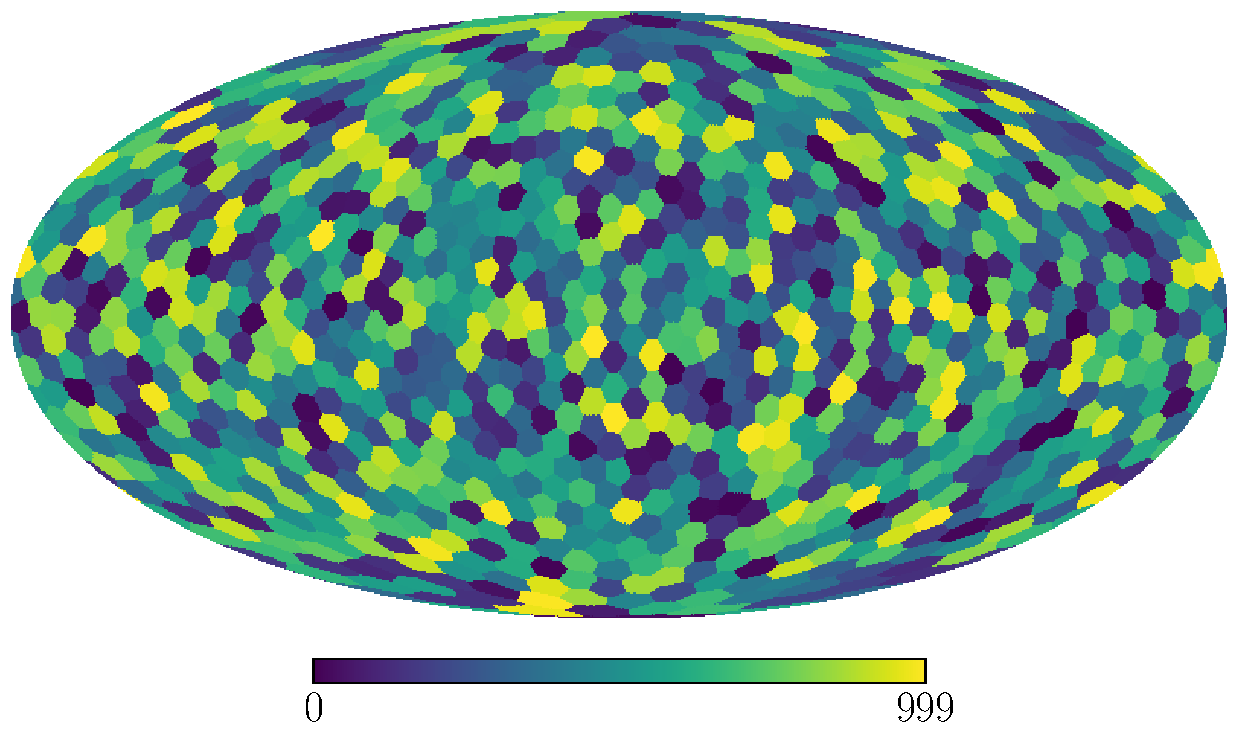
\includegraphics[width=\linewidth]{figures/kmeans_clustering.pdf}
    \caption{Example of spherical K-means clustering applied to a HEALPix-formatted dust map, showing regions sharing a common spectral parameter. Each color represents a distinct cluster.}
    \label{fig:kmeans_clusters}
\end{figure}


In practice, we initialize the clustering of sky pixels using predefined templates such as the Planck Galactic masks (e.g., \texttt{GAL020}, \texttt{GAL040})~\citep{PLANCK}. These masks divide the sky into regions with different levels of Galactic foreground contamination—typically distinguishing low-, medium-, and high-foreground areas based on Galactic latitude or emission intensity thresholds.
Each clustering configuration—defined by the number of patches used for parameters like \( \beta_d \), \( T_d \), and \( \beta_s \)—specifies a distinct model within the data framework of Equation~\eqref{eq:data_model}. Rather than optimizing the clustering assignments directly, we evaluate a grid of such configurations by computing the spectral likelihood in Equation~\eqref{eq:spectral_likelihood} for each mask, selecting the one that minimizes the variance of the recovered CMB.

\subsection{Grid Search over Clustering Models}
\label{subsec:grid_search}

Our model allows the clustering of different spectral parameters (e.g., dust and synchrotron) on independent sets of sky patches, without requiring them to align spatially. The number of clusters assigned to each spectral parameter is treated as a discrete modeling choice, assumed specifically for the purpose of component separation. For example, one configuration might use 100 patches for \( \beta_d \), 20 patches for \( T_d \), and 10 patches for \( \beta_s \).

Letting \( \mathcal{G} \) denote the space of possible clustering configurations:
\[
\mathcal{G} = \{K_{\beta_d} \} \times \{ K_{T_d} \} \times \{ K_{\beta_s} \},
\]
we perform a structured grid search across \( \mathcal{G} \), evaluating each configuration \( \{ \mathcal{C}_k \} \in \mathcal{G} \) by fitting spectral parameters \( \boldsymbol{\beta} \) and reconstructing the CMB component. Specifically, we maximize the spectral likelihood:
\[
\mathcal{L}_{\text{spec}}(\boldsymbol{\beta}, \{ \mathcal{C}_k \}),
\]
where the likelihood depends on both the parameter values and the spatial clustering structure.

Maximizing the spectral likelihood ensures a good fit to the observed frequency maps. However, it does not by itself prevent overfitting, especially when increasing the number of free parameters by introducing finer spatial patching. In low signal-to-noise regions, overly flexible models can fit noise realizations rather than true sky signals, increasing statistical residuals in the reconstructed CMB map.

To mitigate this, we define a secondary selection metric—based on the variance of the reconstructed CMB across noise realizations (described in Section~\ref{subsec:variance_minimization}). The CMB variance acts as a proxy for statistical residuals: minimizing it leads to reduced noise-induced contamination and more robust recovery of the underlying cosmological signal. Thus, the optimal clustering configuration is chosen to balance spectral fit quality with minimization of statistical uncertainty.

Each configuration is assessed over multiple noise realizations and sky regions, ensuring that the selected model is both statistically stable and robust against noise-driven biases.

Given the large size of the configuration space and the need to evaluate multiple noise realizations and sky regions, we developed a distributed, parallel evaluation framework, described next.


\subsection{Distributed and Parallel Execution}
\label{subsec:parallel_grid_search}

To evaluate large grids of clustering configurations across multiple noise realizations and sky regions, we developed a distributed optimization engine: \texttt{jax-grid-search}~\citep{kabalan2025jaxgridsearch}. This \texttt{JAX}-native framework enables high-throughput exploration of parametric component separation models at scale, fully leveraging modern GPU architectures.

As defined previously, the grid \( \mathcal{G} \) spans combinations of patch counts across spectral parameters. 

Each element in this grid represents a distinct clustering configuration. For every such configuration, we evaluate the component separation pipeline across multiple noise realizations and sky regions.

To handle this computational load efficiently, we combine two forms of parallelism:
\begin{itemize}
    \item Intra-device parallelism via \texttt{jax.vmap}, enabling batched execution of component separation fits on a single GPU.
    \item Inter-device parallelism using MPI-style slicing: the global parameter grid is evenly partitioned across all processes, regardless of whether the number of combinations is divisible by the number of workers.
\end{itemize}

Formally, for \( P \) total processes, each process \( I \in [0, P-1] \) is assigned a contiguous chunk of the global grid:
\[
\mathcal{G}_I = \mathcal{G} \left[ \left\lfloor \frac{I \cdot N}{P} \right\rfloor : \left\lfloor \frac{(I+1) \cdot N}{P} \right\rfloor \right], \quad N = |\mathcal{G}|
\]

This ensures robust workload distribution, load balancing, and fault tolerance. It avoids assumptions about grid divisibility and gracefully handles incomplete or interrupted runs—making it well suited for large-scale HPC deployments.

Each batch is independently evaluated, with results checkpointed to disk for aggregation and analysis. This modular design supports recovery, progress tracking, and reproducibility—all essential for exploratory model selection pipelines.
\subsection{Clustering Objective: Variance Minimization}
\label{subsec:variance_minimization}

Let \(\{\mathcal{C}\}\) denote the set of all clustering configurations evaluated in our grid search, and let \(\mathcal{C}_k \in \{\mathcal{C}\}\) denote an individual configuration.

For each clustering configuration in our grid, we perform maximum likelihood estimation of the spectral parameters:
\begin{equation}
\label{eq:grid_search}
\forall\, \mathcal{C}_k \in \{\mathcal{C}\} : \quad \boldsymbol{\beta}_k^* = \arg \max_{\boldsymbol{\beta}_k} \, \mathcal{L}_{\mathrm{spec}}(\boldsymbol{\beta}_k, \mathcal{C}_k)
\end{equation}

Using these parameters, we reconstruct the sky components via:


\begin{align}
\hat{\mathbf{s}} &= \left( \mathbf{A}(\boldsymbol{\beta}_k^*)^\top \mathbf{N}^{-1} \mathbf{A}(\boldsymbol{\beta}_k^*) \right)^{-1} \mathbf{A}(\boldsymbol{\beta}_k^*)^\top \mathbf{N}^{-1} \mathbf{d} \label{eq:recon_operator} \\
                 &\equiv W(\mathbf{d})
\end{align}

From the reconstructed components, we extract the CMB signal \( \hat{s}_{\mathrm{CMB}} \). We compute its variance across noise realizations and average over sky pixels to obtain the scalar objective:
\begin{equation}
\label{eq:min_var}
    \sigma^2_{\mathrm{CMB}} = \left\langle \mathrm{Var}_{i} \left[ \hat{s}^{(i)}_{\mathrm{CMB}} \right] \right\rangle_{\text{pixels}}
\end{equation}

\je{We should probably say we explore other loss functions as well}

Although the spectral parameters \( \boldsymbol{\beta} \) are defined in a clustered fashion—varying across spatial regions—the reconstructed components \( \hat{\mathbf{s}} \), and hence \( \hat{s}_{\mathrm{CMB}} \), are evaluated as a full-sky solution.

This variance serves as the loss function for selecting the best clustering configuration. It acts as a proxy for residual foreground contamination and directly impacts the uncertainty on the inferred tensor-to-scalar ratio \( r \).

Minimizing this variance reduces both statistical uncertainty and systematic leakage in the \( B \)-mode power spectrum. As shown in \citep{Errard2015}, residuals from imperfect foreground modeling propagate into biases on \( C_\ell^{BB} \), making this metric critical for achieving robust and unbiased cosmological constraints.

\subsection{The FURAX Framework}

To support this method, we introduce \texttt{FURAX}~\citep{FURAX}---a modular \texttt{JAX}-powered framework to express and optimize parametric component separation likelihoods.

FURAX is built around a central goal: to express symbolic algebraic expressions (e.g., likelihoods) directly in code using modular, composable operators. These operators abstract common structures like the mixing matrix, noise weighting, or parameter dispatching, and can be combined into scalable computation graphs.

The key features are:
\begin{itemize}
    \item Differentiable algebraic operators for the \textit{mixing matrix} \( \mathbf{A}(\boldsymbol{\beta}) \), the \textit{noise diagonal} operator \( \mathbf{N}^{-1} \), and cluster-wise \textit{SED parameter dispatch} using mask-based routing.
    \item Conjugate gradient solvers via the \texttt{Lineax} library~\citep{lineax} to solve inverse systems efficiently without explicitly forming matrices.
    \item Fully vectorized execution across simulation ensembles and clustering grids, leveraging \texttt{JAX}~\citep{JAX} for efficient large-scale computation.
\end{itemize}

All core computations in FURAX are implemented using memory-efficient linear operators, avoiding explicit dense matrices. This symbolic and modular approach allows \texttt{FURAX} to express and optimize large, realistic models without the memory bottlenecks associated with explicit matrix construction. Ongoing companion developments include forthcoming works on HWP modeling (Tsang King Sang et al.), the MegaTop pipeline (Beringue et al.), the map-maker (Sohn et al.), spherical harmonic tooling (Bazyrov et al., in prep), and extended forecast studies (Villarrubia-Aguilar et al.).


In the scope of this paper, we assume isotropic white noise and matched beam resolution. Although advanced treatments (e.g., beam convolution, correlated noise) exist in the literature, they are not our focus here. However, \texttt{FURAX} is designed to make such extensions straightforward in future developments, including applications to map-making, half-wave plate systematics, atmospheric effects, and beyond.

The framework integrates natively with the \texttt{JAX} ecosystem and supports optimization and inference workflows through libraries such as \texttt{Optax}~\citep{optax} and \texttt{NumPyro}~\citep{numpyro}.

\begin{figure}
    \centering
    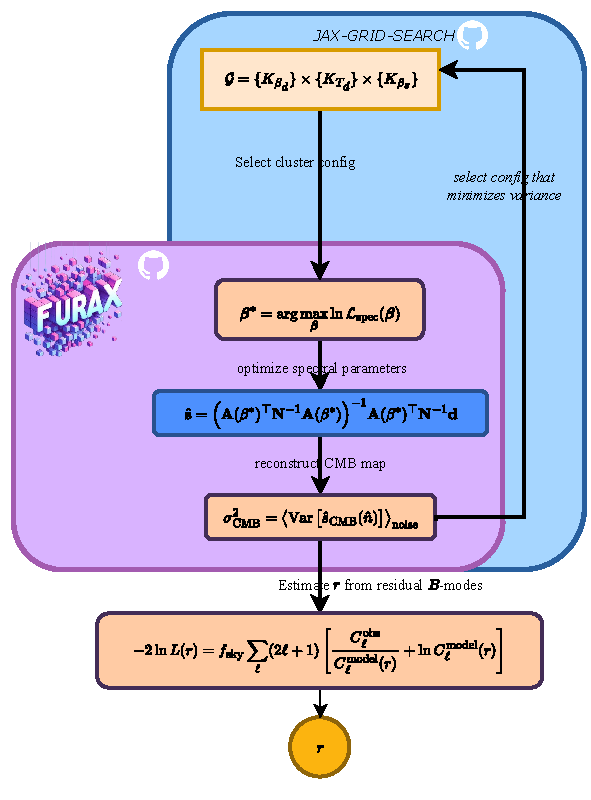
\includegraphics[width=\linewidth]{figures/FURAX-CS.pdf}
    \caption{
        Overview of the \texttt{FURAX} pipeline for component separation and tensor-to-scalar ratio estimation. The process begins by selecting a clustering configuration from the discrete grid \( \mathcal{G} = \{K_{\beta_d}\} \times \{K_{T_d}\} \times \{K_{\beta_s}\} \), evaluated in parallel using \texttt{JAX-GRID-SEARCH}. Each configuration undergoes spectral parameter optimization and map reconstruction using \textsc{FURAX}. The variance \je{or other loss function?} of the recovered CMB map is used as a selection metric to identify the best configuration. The final CMB map is then used to compute the \( B \)-mode power spectrum and infer the tensor-to-scalar ratio \( r \). 
    }
    \label{fig:furax_pipeline}
\end{figure}

\section{Spectral Likelihood Maximization}

The central task in parametric component separation is the estimation of spectral parameters \( \boldsymbol{\beta} \) by maximizing the spectral likelihood \( \mathcal{L}_{\mathrm{spec}}(\boldsymbol{\beta}) \)~\eqref{eq:spectral_likelihood}. This likelihood serves as the objective function that drives parameter inference across the model.

Thanks to \texttt{JAX}'s automatic differentiation, gradients of this objective with respect to all free parameters are computed efficiently. This applies even in spatially varying models, where spectral parameters are defined per cluster and must be dispatched to the appropriate sky pixels. Crucially, this indexing and dispatching operation, performed via binary masks, are themselves implemented in a differentiable manner. As a result, the likelihood function is compatible with gradient-based optimization.

\texttt{FURAX} performs spectral likelihood maximization using gradient-based optimization from the \texttt{Optax} library~\citep{optax}. The default method is L-BFGS \je{add-ref}, a limited-memory quasi-Newton optimizer that leverages curvature information from past gradients. Ideally, optimization would proceed via a full Newton step:
\begin{equation}
    \theta_{n+1} = \theta_n - H^{-1} \nabla L(\theta_n),
\end{equation}
where \( H \) is the Hessian of the loss. However, computing and inverting this matrix becomes intractable for large-scale clustered models with thousands of parameters. L-BFGS avoids this cost by constructing a low-rank approximation using a limited history of gradients and parameter updates, enabling efficient and memory-scalable updates.

In practice, we observe that L-BFGS in \texttt{FURAX} exhibits superior stability and convergence (see Figure~\ref{fig:runtime_comparison}) compared to earlier approaches such as \texttt{FGBuster}. This is primarily due to two factors: (i) we use exact gradients from automatic differentiation in \texttt{JAX}, ensuring consistent and smooth optimization dynamics; and (ii) we avoid the use of Singular Value Decomposition (SVD)~\citep{SVD}, which \texttt{FGBuster} employs as a performance shortcut at the cost of numerical noise in gradients. These design choices make \texttt{FURAX} robust to initialization and capable of converging reliably even in high-dimensional, highly clustered configurations.

We also experimented with TNC (Truncated Newton with Constraints)~\citep{TNC}, as used in \texttt{FGBuster}. In our framework, TNC is accessed through \texttt{jaxopt}~\citep{jaxopt}, which wraps \texttt{scipy.optimize.minimize}~\citep{scipy}. However, this implementation runs exclusively on CPU and is incompatible with \texttt{JAX}’s \texttt{jit} compilation or \texttt{vmap} vectorization. More critically, TNC does not scale well with parameter count---as the number of clusters increases, the optimization problem becomes stiff and memory-bound, leading to significantly longer runtimes and poorer convergence behavior.

First-order optimizers such as Adam~\citep{adam} were also tested, but proved to be ill-suited for this application. Adam applies a uniform learning rate schedule across all parameters, yet in component separation, the physical scales of spectral parameters differ substantially: for instance, \( \beta_d \) varies between 0.5 and 5, \( T_d \) between 10 and 50\,\(\mathrm{K}\), and \( \beta_s \) between \(-6\) and \(-1\).

Moreover, the spectral likelihood typically reaches values on the order of \( 10^8 \) (for example, at nside \( 64 \)) \je{at an Healpix (ref) nside= 64}, making fixed or scheduled learning rates ineffective. In contrast, L-BFGS employs a line search strategy that dynamically adapts the step size to local curvature, enabling stable convergence even in high-dimensional, multi-scale optimization settings.

\begin{figure}
\centering
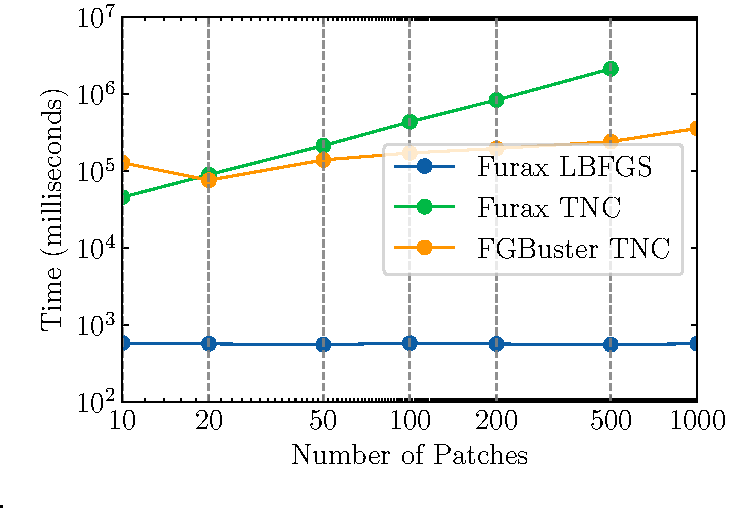
\includegraphics[width=1\columnwidth]{figures/runtime_comparison.pdf}
\caption{Runtime comparison of \texttt{FGBuster} (TNC), \texttt{FURAX} (TNC) using \texttt{jaxopt}, and \texttt{FURAX} (L-BFGS) using \texttt{optax} as a function of the number of clusters. L-BFGS scales robustly with parameter count and consistently outperforms TNC in clustered models. }
\label{fig:runtime_comparison}
\end{figure}

\section{Tensor-to-Scalar Ratio Estimation}
\label{sec:r_estimation}

We estimate the tensor-to-scalar ratio \( r \) from the \( B \)-mode power spectrum of the reconstructed CMB maps. The process involves modeling residual contamination, combining it with signal templates, and performing likelihood-based inference of \( r \)~\citep{STOMPER16, ERRAR18}.

To ensure statistical robustness, the full estimation pipeline is applied across multiple noise realizations and distinct sky regions. The resulting B-mode power spectra and corresponding likelihoods are then averaged over both axes, the noise and the sky region, to account for sample variance and foreground complexity.

\je{this probably does not deserve a numbered paragraph}
\paragraph{BB Spectrum Convention.}
All angular power spectra are reported in the standard units:
\[
\text{coeff} = \frac{\ell(\ell + 1)}{2\pi},
\]


\paragraph{Systematic and Statistical Residuals.}
To quantify contamination in the recovered CMB, we separate residuals into two components:
\begin{itemize}

    \item Systematic residual power is obtained by rerunning the full component separation pipeline on foreground-only skies \( d_{\mathrm{ds}} \), which exclude both CMB and instrumental noise. This evaluates the imprint of foreground leakage that cannot be filtered out by the model:
    \begin{equation}
    C_\ell^{\mathrm{syst}} = C_\ell \left( W(d_{\mathrm{ds}}) \right),
    \end{equation}
    where \( W \) denotes the reconstruction operator as defined in~\eqref{eq:recon_operator}. The resulting residuals capture systematic foreground contamination intrinsic to the modeling assumptions and patch structure.

    \item Total residual power is computed from the full reconstruction error across noise realizations:
    \begin{equation}
    C_\ell^{\mathrm{res}} = \left\langle C_\ell \left( \hat{s}_{\mathrm{CMB}}^{(n)} - s_{\mathrm{CMB}}^{\mathrm{true}} \right) \right\rangle_{n},
    \end{equation}
    where \( n \) indexes the noise realizations and \( \hat{s}_{\mathrm{CMB}}^{(n)} \equiv W(d^{(n)}) \).
    This represents the total error power, including residual foregrounds and instrumental noise.

    \item Statistical residual power, due solely to instrumental noise, is extracted by subtraction:
    \begin{equation}
    C_\ell^{\mathrm{stat}} = C_\ell^{\mathrm{res}} - C_\ell^{\mathrm{syst}}.
    \end{equation}
\end{itemize}
This decomposition isolates stochastic uncertainty from systematic bias, and \( C_\ell^{\mathrm{stat}} \) is used as the effective noise floor for likelihood estimation.

\paragraph{BB Spectrum Model.}
We model the theoretical \( B \)-mode spectrum as:
\begin{equation}
C_\ell^{BB}(r) = r \cdot C_\ell^{\mathrm{tensor}} + C_\ell^{\mathrm{lensing}} + C_\ell^{\mathrm{stat}},
\end{equation}
where \( C_\ell^{\mathrm{tensor}} \) is a primordial tensor-mode template normalized to \( r = 1 \), \( C_\ell^{\mathrm{lensing}} \) is the fixed lensing \( B \)-mode contribution, and \( C_\ell^{\mathrm{stat}} \) accounts for statistical residuals from noise and imperfect foreground cleaning.

\paragraph{Likelihood and Inference.}
The tensor-to-scalar ratio \( r \) is inferred by maximizing a chi-squared likelihood function under the assumption of Gaussian-distributed residuals:
\begin{equation}
-2 \ln \mathcal{L}_{\mathrm{c}}(r) = f_{\mathrm{sky}} \sum_\ell (2\ell + 1) \left[ \frac{C_\ell^{\mathrm{obs}}}{C_\ell^{\mathrm{model}}(r)} + \ln C_\ell^{\mathrm{model}}(r) \right]
\end{equation}

% pour eviter le leakage il faut 
% shat = c1 + res total 
% res = Shat - c1 (UNSEEN)
% cl res
% Cl OBS = bb_lens + cl res
% CL True = c1 sans mask

We evaluate this function over a grid of \( r \) values and report the best-fit \( \hat{r} \) corresponding to the minimum of the negative log-likelihood. Uncertainties are estimated from the curvature of the likelihood around its maximum.

\section{Results}
\label{sec:results}

\subsection{Validation of the Framework}
\label{subsec:validation}

To assess the performance of our clustered component separation framework, we construct a synthetic validation setup in which the true sky components and spectral parameters are fully known. This controlled environment enables precise measurement of reconstruction quality, residual contamination, and estimator consistency.

The simulation begins by defining a known sky signal \( \mathbf{s} \) in Equation~\eqref{eq:data_model}, consisting of Stokes \( Q/U \) maps for CMB, thermal dust, and synchrotron emission, all specified at a common reference frequency. This sky vector is then mixed using a known mixing matrix \( \mathbf{A}(\boldsymbol{\beta}) \), where \( \boldsymbol{\beta} \) encodes the ground-truth spectral parameters for each component. Table~\ref{tab:validation_config} summarizes the simulation parameters.

The noise vector \( \mathbf{n} \) is sampled as Gaussian white noise, scaled to match LiteBIRD-like polarization depth \je{ref to PTEP} across the frequency channels. Each clustering configuration is evaluated across 100 independent noise realizations to reduce statistical variance and assess estimator stability.

We perform a grid search over discrete cluster configurations (defined in Section~\ref{subsec:grid_search}), varying the number of patches assigned to each spectral parameter. For each setup, we run the full component separation pipeline by minimizing the spectral negative log-likelihood. The resulting CMB map \( \hat{s}_{\mathrm{CMB}} \) is then compared with the input to assess reconstruction fidelity and the accuracy of tensor-to-scalar ratio estimation.

\begin{table}
    \centering
    \small
    \caption{Validation setup used in the synthetic benchmark.}
    \label{tab:validation_config}
    \begin{tabular}{@{}p{3.5cm}|p{5cm}@{}}
        \toprule
        \textbf{Parameter} & \textbf{Value / Range} \\
        \midrule
        Resolution & \( N_{\text{side}} = 64 \) \\
        Sky mask & \texttt{GAL020} \je{add a ref to Planck masks (like ESA data base = where to find them)}\\
        Noise realizations & 100 \\
        Patch count grid & \( \beta_d \in [10, 300] \), \( T_d, \beta_s \in [5, 20] \) \\
        True patch count & \( \beta_d = 100 \), \( T_d = 20 \), \( \beta_s = 20 \) \\
        \bottomrule
    \end{tabular}
\end{table}


Figure~\ref{fig:grid_search_summary} shows the grid search results. The configuration minimizing the CMB variance coincides with the configuration yielding the lowest spectral negative log-likelihood, \je{not sure what you mean here BEGIN} indicating that improved physical reconstruction aligns with optimal statistical fit \je{END}. Importantly, the recovered clustering matches the true simulation setup exactly, validating the robustness of the variance-based selection criterion against noise-driven overfitting.

\begin{figure}
    \centering
    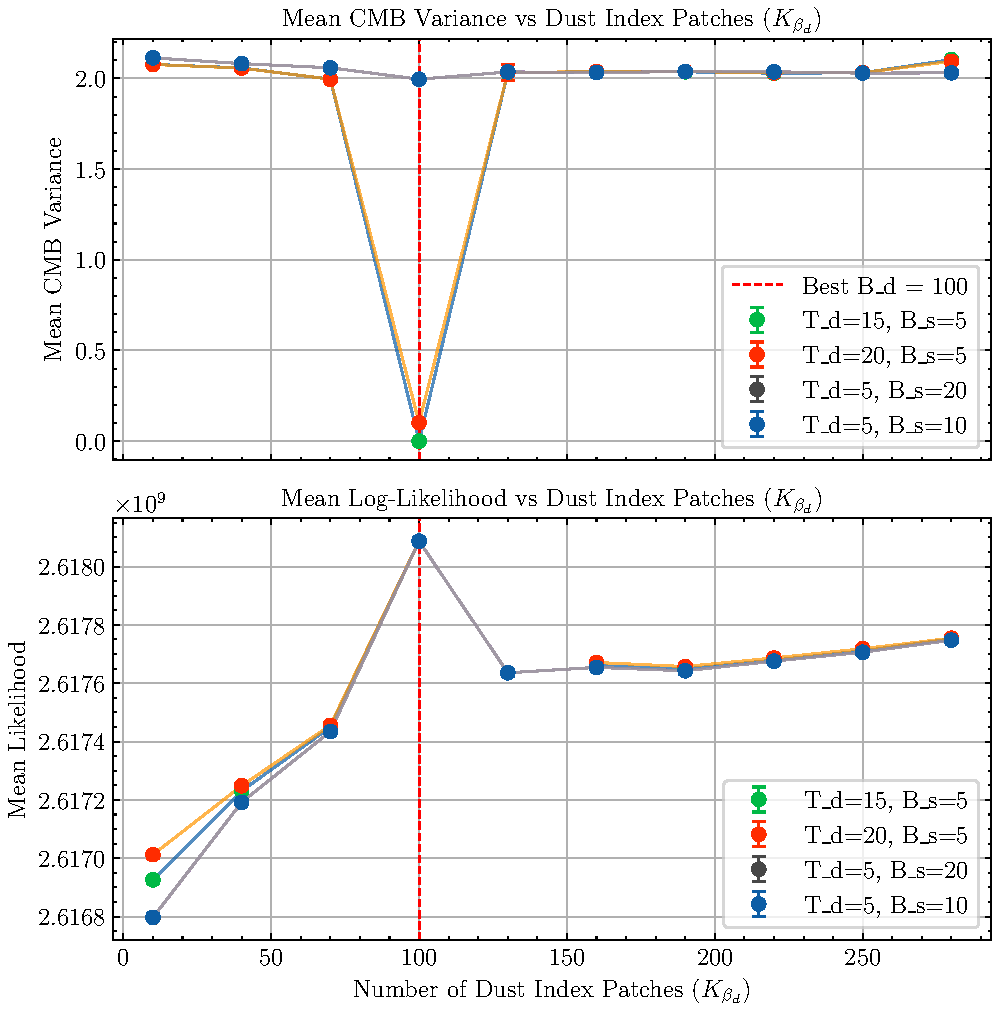
\includegraphics[width=\linewidth]{figures/validation_likelihood_vs_variance.pdf}
    \caption{
    Grid search results for varying number of dust spectral index patches \( K_{\beta_d} \), while keeping other parameters fixed.
    Each curve corresponds to a different configuration of \( K_{T_d} \) and \( K_{\beta_s} \).
    \textbf{Top:} Mean variance of the reconstructed CMB component across noise realizations, used as the primary selection metric \je{could you add error bars corresponding to the scatter of the map variance across noise simulations ?}.
    \textbf{Bottom:} Mean spectral negative log-likelihood, offset for readability.
    The vertical red line marks the true value used in the simulated sky (\( K_{\beta_d} = 100 \)), and the dashed lines indicate the global extrema of each metric.
    The configuration \( K_{\beta_d} = 100 \), \( K_{T_d} = 15 \), and \( K_{\beta_s} = 5 \) was used to generate the reference clustered map.
    Minimizing the CMB variance successfully recovers the true clustering configuration.
    \je{add uK **2 for CMB Variance ?}\\
    \je{for the notation of the number of clusters}\\
    \je{dont you prefer to use notation at the beginnin of section 2.3, e.g. $K_{T_d}$ ? to avoid confusion with the value of Td}
    }

    \label{fig:grid_search_summary}
\end{figure}


\subsection{K-means Clustering vs. Multi-Resolution}
\label{subsec:comparison_setup}

We compare two spatial modeling strategies for parametric component separation, both implemented within the \textsc{FURAX} framework:
\begin{itemize}
    \item \textbf{K-means clustering}, which uses spherical K-means to construct spatial patches over which spectral parameters are common (introduced in Section~\ref{subsec:sph_kmeans}).
    \item \textbf{Multi-resolution grouping}, \je{why not calling it multi-Healpix instead? or multi-nside? 
(because the Kmeans do also lead to "multiresolution" maps anyway ..)} which defines parameter patches by downgrading HEALPix maps to coarser resolutions, following the strategy of~\citep{LiteBIRD_PTEP_2022}~\citep{ERRAR18}.
\end{itemize}

Although applied to the same sky and instrument setup, these approaches differ fundamentally in how they capture spatial variability. The K-means strategy allows a flexible, data-driven exploration of spatial granularity, while the multi-resolution method imposes predefined patch sizes. This comparison evaluates reconstruction fidelity, residual suppression, and consistency in inferred cosmological parameters.

\subsubsection*{Simulation Setup}

Simulated skies are generated using \texttt{PySM3} \je{je pense que "Group" n'est pas le bon nom pour cette citation} ~\citep{Panexp_2025,Zonca_2021,Thorne_2017}, combining CMB, thermal dust, and synchrotron emission (\texttt{c1d1s1} model).

\begin{table}
    \centering
    \small
    \caption{Simulation parameters used for both methods.}
    \label{tab:comparison_sim}
    \begin{tabular}{@{}p{3.5cm}|p{5cm}@{}}
        \toprule
        \textbf{Parameter} & \textbf{Value} \\
        \midrule
        Resolution & \( N_{\text{side}} = 64 \) \\
        Sky model & \texttt{c1d1s1} \\
        Sky mask & \texttt{GAL020} \\
        Instrument & LiteBIRD-like \\
        Noise realizations & 100 per region \\
        \bottomrule
    \end{tabular}
\end{table}

\subsubsection*{Sky Region Partitioning}

To probe performance across different foreground regimes, we define distinct sky zones using Planck-based Galactic masks:

\je{should these two lines be merged in the two other bullet points on the left? not sure why they are separated at the moment}
\begin{itemize}
    \item \textbf{K-means clustering} is applied to six disjoint subregions, obtained by splitting each mask into upper and lower hemispheric parts: \texttt{GAL020\_U}, \texttt{GAL020\_L}, \texttt{GAL040\_U}, \texttt{GAL040\_L}, \texttt{GAL060\_U}, and \texttt{GAL060\_L}.
    \item \textbf{Multi-resolution grouping} \je{similarly to what is done in PTEP (2023)} is applied separately to the full-sky masks: \texttt{GAL020}, \texttt{GAL040}, and \texttt{GAL060}.
\end{itemize}

These masks span from high Galactic latitudes (low foregrounds, \texttt{GAL020}) to regions closer to the Galactic plane (higher foregrounds, \texttt{GAL060}); see Figure~\ref{fig:mask_layout}.


\begin{figure}
    \centering
    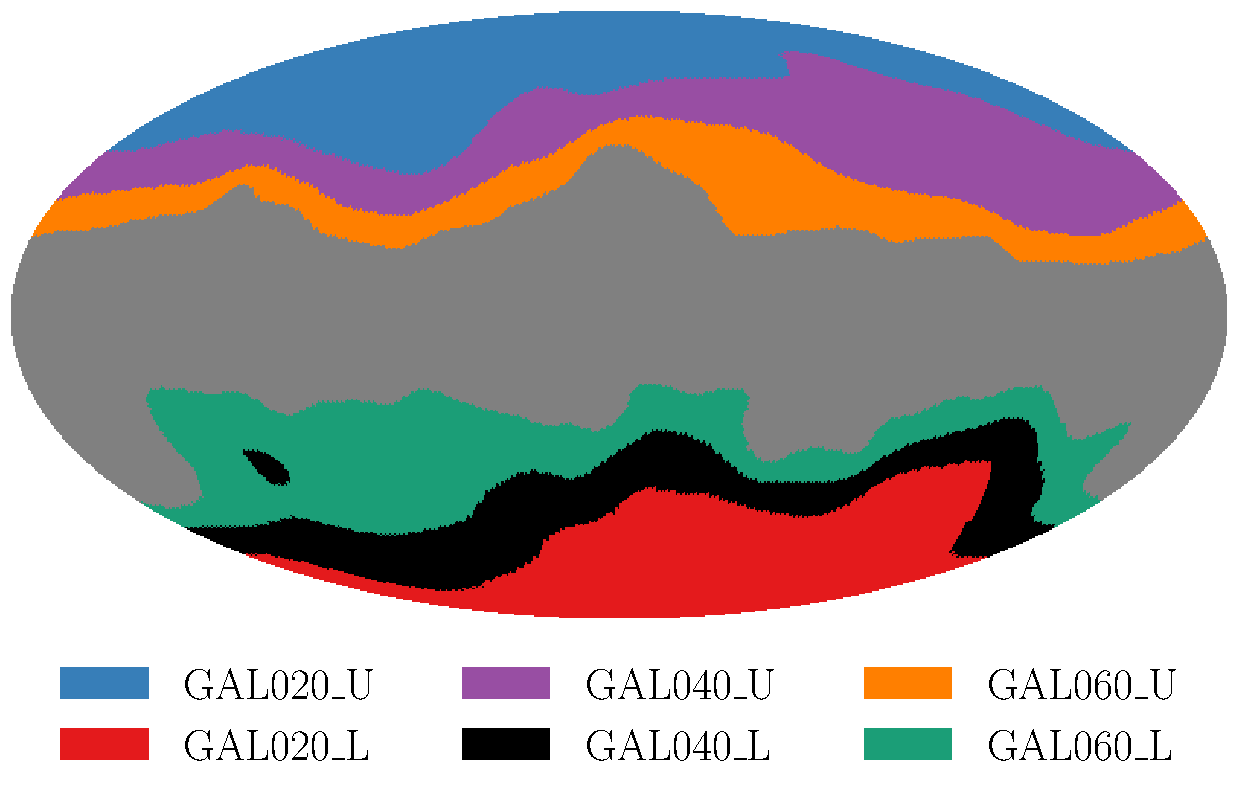
\includegraphics[width=\linewidth]{figures/sky_region_mask_zones.pdf}
    \caption{
    Sky regions used in the comparison study. 
    Colored areas correspond to the six disjoint regions for adaptive clustering.
    These masks are based on the Planck Galactic masks~\citep{Planck2015Galactic}.
    }
    \label{fig:mask_layout}
\end{figure}

\subsubsection*{Grid-Search Clustering}

\je{BEGIN : not sure this sentence is necessary?}
In the adaptive clustering approach, spectral parameters are assigned to pixel clusters defined via spherical K-means \je{END}. A structured grid search over patch counts is performed, selecting the configuration that minimizes the CMB variance across 100 noise realizations. This fully data-driven search avoids assumptions about spatial scales and allows optimal patch sizes to emerge from the data itself.

\begin{table}
    \centering
    \small
    \caption{Grid-search clustering configuration.}
    \begin{tabular}{@{}p{3.8cm}|p{4.5cm}@{}}
        \toprule
        \textbf{Parameter} & \textbf{Patch Count Range} \\
        \midrule
        \( \beta_d \) & 100 to 5000 (in steps of 100) \\
        \( T_d \), \( \beta_s \) & \{1, 5, 20, 30, 50, 60, 70, 80\} \\
        Sky regions & Six zones (\texttt{GAL020\_U}, etc.) \\
        Noise realizations & 100 per region \\
        \bottomrule
    \end{tabular}
\end{table}

\subsubsection*{Multi-Resolution Grouping}

The multi-resolution grouping method creates spatial patches by degrading the original HEALPix pixelization to coarser \( N_{\text{side}} \) values, separately for each spectral parameter. After patching, the maps are upsampled back to \( N_{\text{side}} = 64 \) to match the data grid.

\begin{figure}
    \centering
    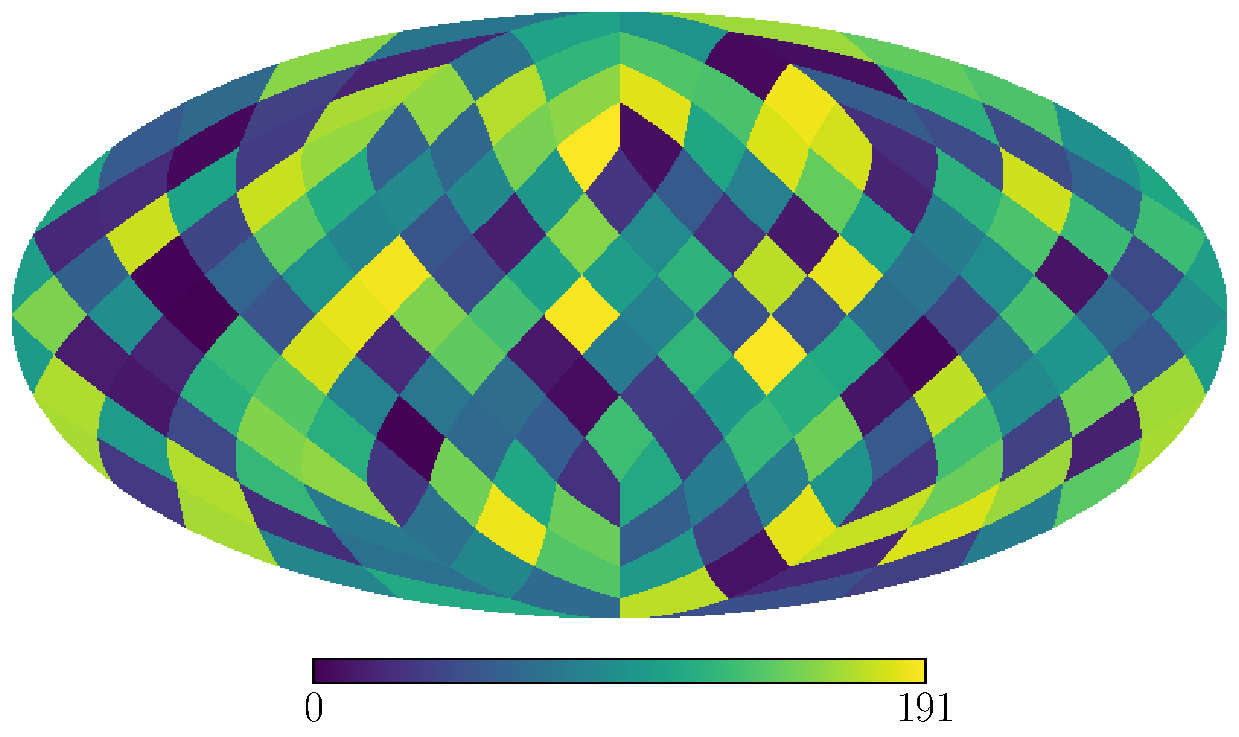
\includegraphics[width=0.9\linewidth]{figures/multi_resolution_pixel_grouping.pdf}
    \caption{Multi-resolution mega-pixel structure. Example showing downgraded patch regions from \( N_{\text{side}} = 64 \) to \( N_{\text{side}} = 8 \).}
    \label{fig:multires_megapixels}
\end{figure}

The patching resolutions vary depending on the sky mask and spectral parameter, as summarized in Table~\ref{tab:multires_config}. These configurations follow the multi-resolution grouping scheme used in~\citep{LiteBIRD_PTEP_2022}.

\begin{table}
    \centering
    \small
    \caption{Multi-resolution configuration per mask region (used in the main experiments).}
    \begin{tabular}{@{}p{3.5cm}|p{1.5cm}@{}|p{1.5cm}@{}|p{1.5cm}@{}}
        \toprule
        \textbf{Region (Mask)} & \( \beta_d \) & \( T_d \) & \( \beta_s \) \\
        \midrule
        \texttt{GAL060} (low lat.)  & 64 & 8 & 4 \\
        \texttt{GAL040} (mid lat.)  & 64 & 4 & 2 \\
        \texttt{GAL020} (high lat.) & 64 & 0 & 2 \\
        \bottomrule
    \end{tabular}
    \label{tab:multires_config}
\end{table}

\begin{table}
    \centering
    \small
    \caption{Alternative multi-resolution configurations used for validation.}
    \begin{tabular}{@{}p{3.5cm}|p{1.5cm}@{}|p{1.5cm}@{}|p{1.5cm}@{}}
        \toprule
        \textbf{Region (Mask)} & \( \beta_d \) & \( T_d \) & \( \beta_s \) \\
        \midrule
        \texttt{GAL060} (low lat.)  & 64 & 8 & 8 \\
        \texttt{GAL040} (mid lat.)  & 64 & 4 & 4 \\
        \texttt{GAL020} (high lat.) & 64 & 0 & 4 \\
        \bottomrule
    \end{tabular}
    \label{tab:multires_config}
\end{table}

While computationally efficient, this fixed-resolution approach lacks the flexibility to adapt to localized foreground complexity, which explains the superior reconstruction performance achieved by adaptive clustering.

\subsection{Runtime and Parallelization}
\label{subsec:runtime}

The extensive clustering and component separation runs were performed on the \textit{Jean Zay} supercomputer \je{add ref for jean zay}, utilizing NVIDIA A100 GPUs distributed across 4 compute nodes (32 GPUs total). Computations were executed using the \texttt{jax-grid-search} framework (Section~\ref{subsec:parallel_grid_search}), leveraging JAX's native parallelization capabilities for high-throughput evaluation.

The full study encompassed:
\begin{itemize}
    \item 3200 clustering configurations,
    \item each evaluated across 100 independent noise realizations,
    \item over 6 distinct sky regions (Figure~\ref{fig:mask_layout}),
\end{itemize}
leading to approximately 1.92 million independent component separation runs.

Despite the large computational volume, the full grid was scanned in under 30 hours, consuming approximately 1000 GPU-hours. For comparison, earlier CPU-based frameworks such as \texttt{FGBuster} required around 40 minutes per configuration, making such exhaustive parameter scans practically infeasible.

This performance gain stems from two key design choices: (i) extensive batching and vectorization of likelihood evaluations within each GPU, and (ii) distributed slicing of the grid across multiple devices without assuming divisibility. The implementation supports checkpointing, failure recovery, and fully reproducible execution, ensuring robustness for large HPC deployments.

Thanks to this scalability, \texttt{FURAX} enables a new regime of data-driven model selection, where clustering hypotheses are tested systematically across noise realizations and sky regions, rather than being fixed a priori.

\subsection{CMB Reconstruction Comparison}
\label{subsec:cmb_reconstruction}

We assess the CMB reconstruction performance achieved by the two spatial modeling strategies introduced in Section~\ref{subsec:comparison_setup}: clustering-based patching via K-means and fixed-resolution multi-resolution grouping. Both methods are applied to the same simulated sky (CMB plus foregrounds) with LiteBIRD-like noise and angular resolution. \je{BEGIN : this should probably go earlier when simulations are detailed} Beam effects are not modeled in this comparison, as the analysis is restricted to low-resolution simulations with \( N_{\text{side}} = 64 \). \je{END}


The analysis focuses on the accuracy of the reconstructed CMB polarization fields, examining both Stokes \( Q \) and \( U \) components, and on quantifying residual foreground leakage.

\vspace{2mm}

\subsubsection*{Patch Structures}
Before presenting reconstruction results, we first illustrate the spatial patch layouts produced by each method. Figures~\ref{fig:furax_patches} and~\ref{fig:multires_patches} show the pixel clustering \je{the optimal pixel clustering -- obtained after minimizing variance?} for the three spectral parameters: \( \beta_d \), \( T_d \), and \( \beta_s \).

The K-means clustering approach (Figure~\ref{fig:furax_patches}) produces flexible, equal-area patches that adapt to the local sky complexity by minimizing the CMB variance. In contrast, the multi-resolution method (Figure~\ref{fig:multires_patches}) relies on a fixed HEALPix downgrading scheme, imposing uniform patch sizes across large sky regions.

From the results shown in Figure~\ref{fig:furax_patches}, we find that the optimal patch count for our setup was 1500 for both the synchrotron spectral index \( \beta_{\mathrm{s}} \) and the thermal dust temperature \( T_{\mathrm{dust}} \), compared to 343 and 144, respectively, in the multi-resolution scheme (Figure~\ref{fig:multires_patches}). The dust spectral index \( \beta_d \) was modeled as a per-pixel parameter in both methods.

These structural differences in patching strongly influence the quality of component separation, as discussed in the following sections.

\begin{figure}
    \centering
    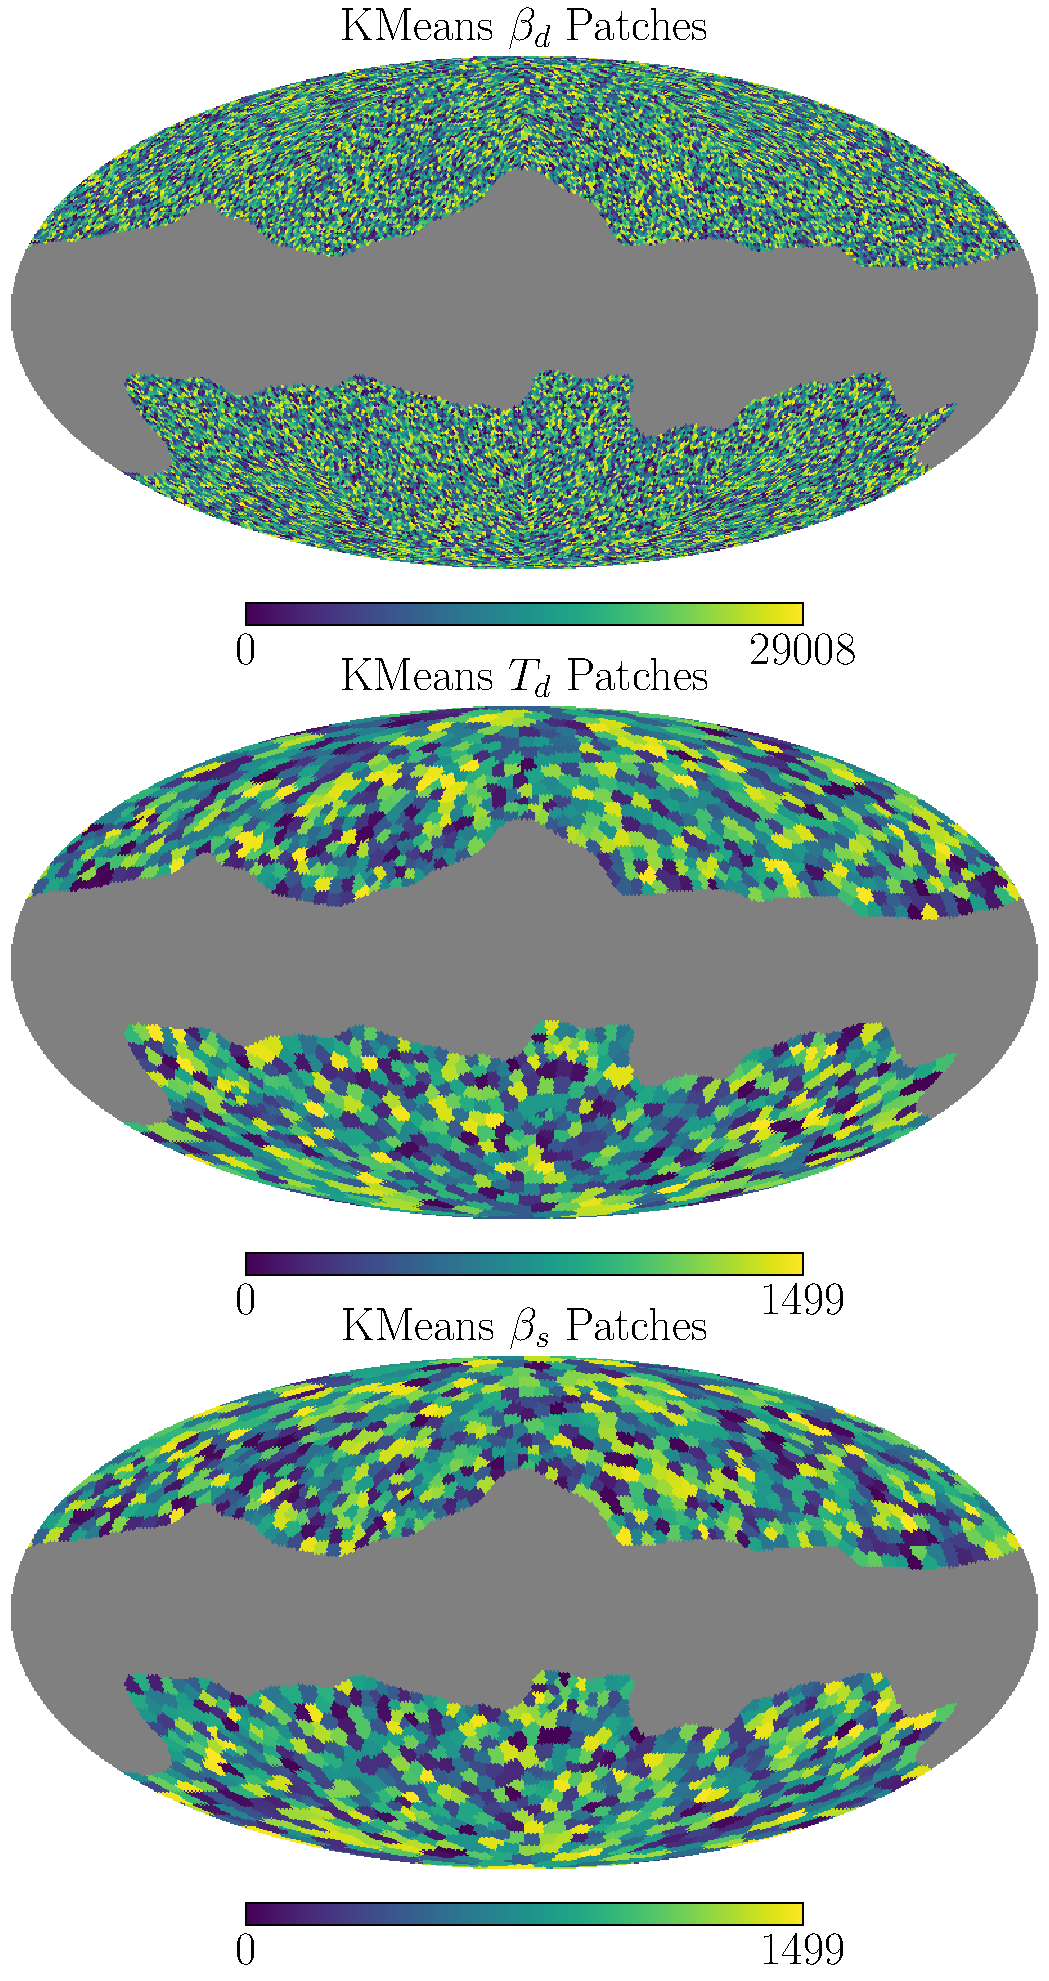
\includegraphics[width=\linewidth]{figures/kmeans_patch_layout.pdf}
    \caption{
    Final FURAX clustering configuration. 
    Top to bottom: patches for \( \beta_d \), \( T_d \), and \( \beta_s \), obtained by grid search minimizing the CMB reconstruction variance.
    The clusters are irregular and data-driven, adapting to spatial variations in the foreground complexity.
    }
    \label{fig:furax_patches}
\end{figure}

\begin{figure}
    \centering
    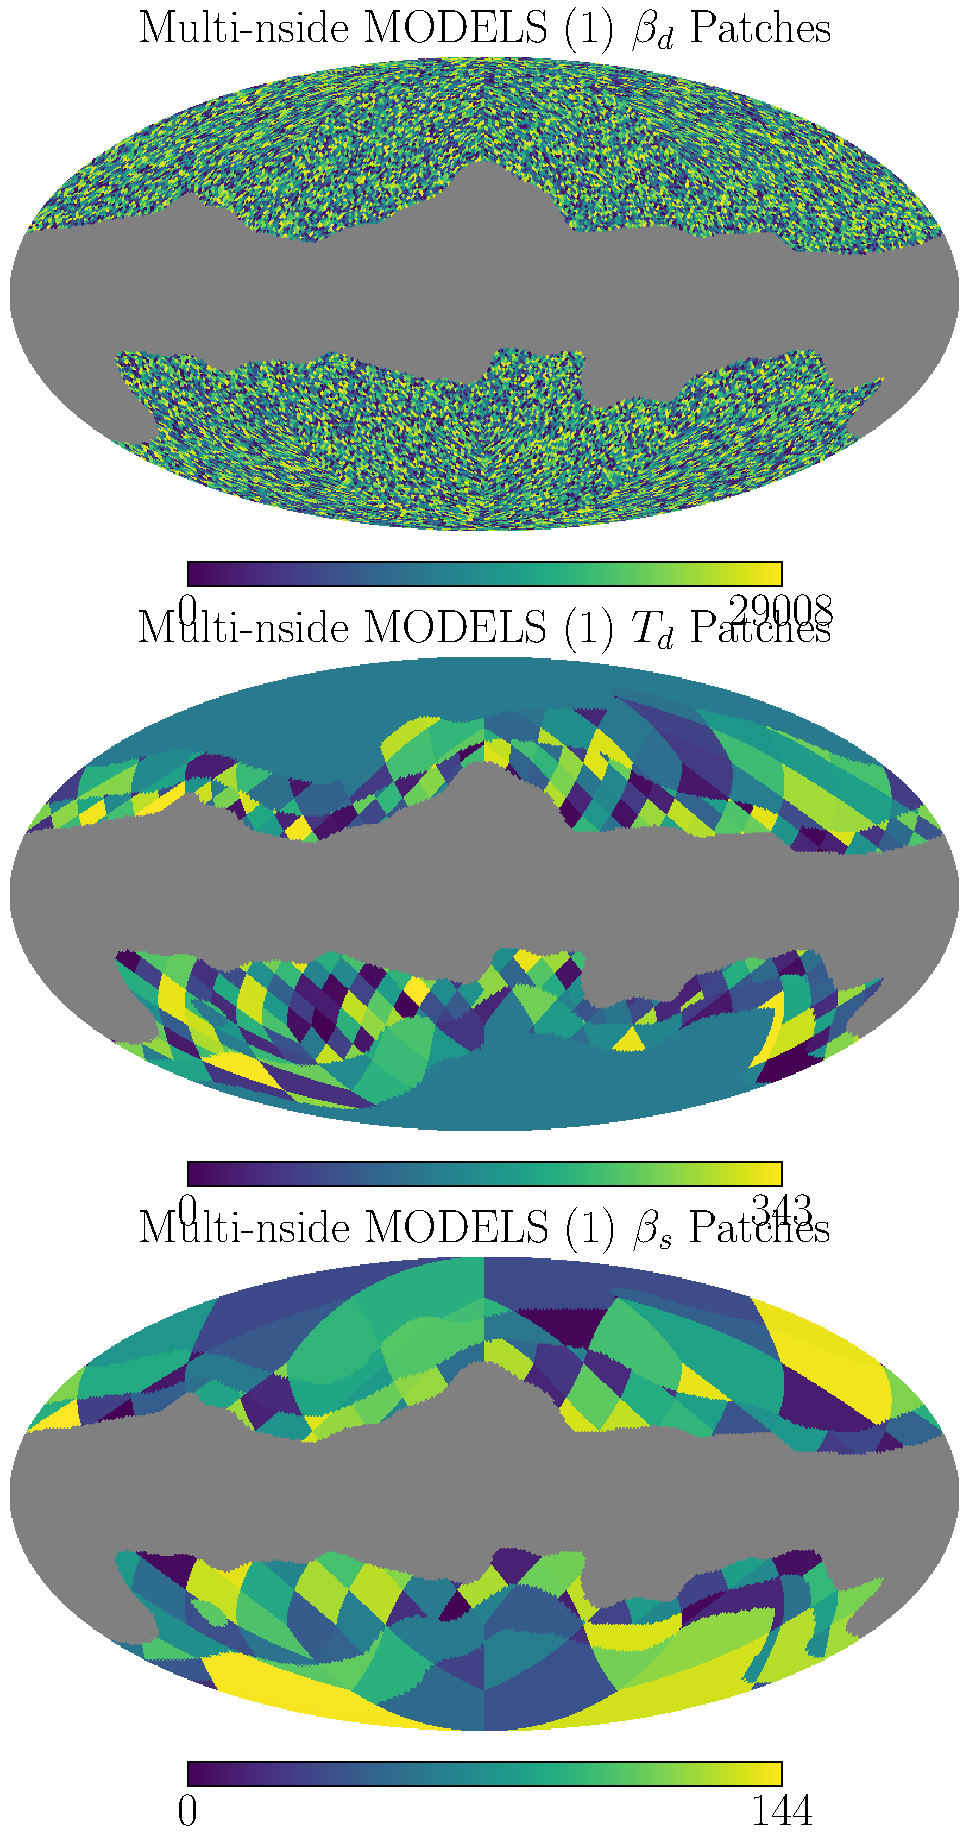
\includegraphics[width=\linewidth]{figures/multires_patch_layout.pdf}
    \caption{
    Multi-resolution patch structure.
    Top to bottom: groupings for \( \beta_d \), \( T_d \), and \( \beta_s \), generated by downgrading HEALPix maps to fixed \( N_{\text{side}} \) resolutions.
    The patches are regular and uniform, independent of the true sky variability.
    This corresponds to table \ref{tab:multires_config}.
    }
    \label{fig:multires_patches}
\end{figure}



%% HI
\subsection{Residuals and CMB Reconstruction}
\label{sec:residuals_reconstruction}

We assess the quality of CMB reconstruction achieved by the three spatial modeling strategies: single-patch \je{to be introduced maybe, I think this is the first time it appears}, multi-resolution, and K-means clustering.  
The evaluation focuses separately on:
\begin{itemize}
    \item Residual CMB polarization maps (\( Q \) and \( U \))
    \item Residual \( B \)-mode power spectra \je{B-modes angular power spectrum of residuals?}
\end{itemize}

We first examine the residual maps, defined as the difference between the reconstructed and true CMB polarization fields for Stokes \( Q \) and \( U \).

Figure~\ref{fig:cmb_qu_comparison} compares the results across methods.

The multi-resolution approach achieves the visually cleanest maps, with minimal foreground residuals across the sky.  
K-means clustering yields slightly larger residuals but still substantially improves over the single-patch baseline, which shows significant large-scale errors.  
These results illustrate the benefits of spatially adaptive modeling; however, as we will discuss in the next section, lower visual residuals do not necessarily imply better statistical performance at the power spectrum level.

\begin{figure*}
    \centering
    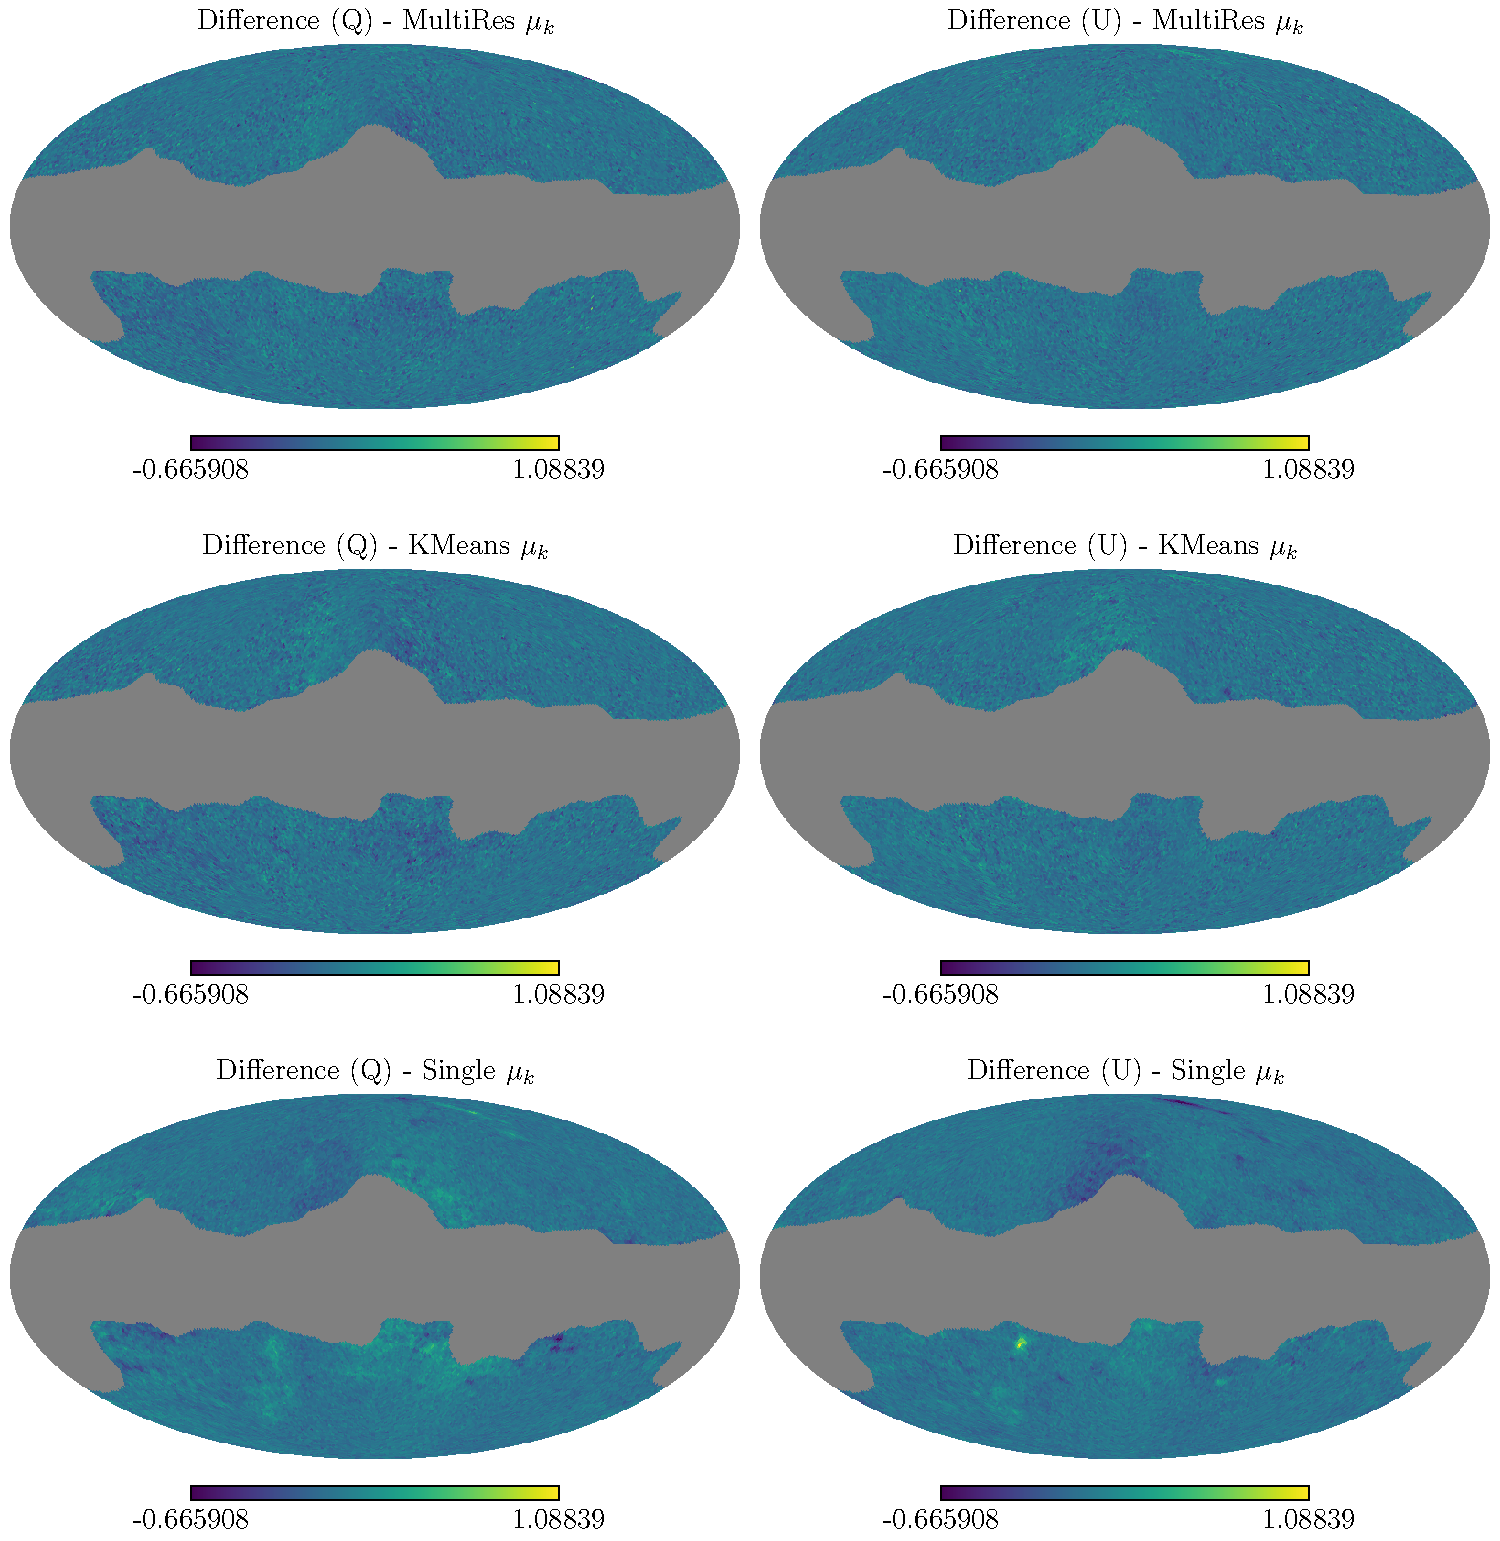
\includegraphics[width=\linewidth]{figures/cmb_recon.pdf}
    \caption{
    Residual CMB polarization maps (Stokes \( Q \) and \( U \)) for single-patch, multi-resolution table~\ref{tab:multires_config}, and K-means clustering methods.  
    While multi-resolution yields the lowest mean squared error (MSE)—with MSE\(_Q = 6.7 \times 10^{-4}\) $\mu_k²$, MSE\(_U = 4.6 \times 10^{-4}\)$\mu_k²$ , K-means performs only slightly worse \je{do we understand how that can be the case? isn't Kmeans bound to always do better than healpix ?} (MSE\(_Q = 8.0 \times 10^{-4}\)$\mu_k²$ , MSE\(_U = 5.5 \times 10^{-4}\))$\mu_k²$,  but substantially outperforms the single-patch model. 
    The small sacrifice in pixel-level reconstruction accuracy is offset by improved control of residual foregrounds—consequently giving a less biased estimation oftensor the tensor-to-scalar ratio \( r \).
    }
    \label{fig:cmb_qu_comparison}
\end{figure*}

\subsubsection*{Residual \( B \)-Mode Power Spectra}
\label{subsec:residual_bb_spectra}

We now decompose the residuals into systematic and statistical contributions at the level of the \( B \)-mode angular power spectrum.

Figure~\ref{fig:bb_spectra_comparison} shows the residual spectra across all multipoles.  
To contextualize the scale of residual contamination, we also plot the theoretical \( B \)-mode power spectra from lensing and primordial tensor modes (\( r=1 \)) \je{you used r=0.001 in the figure}, computed using the CAMB python package~\citep{CAMB}.

This confirms that minimizing the CMB variance through adaptive clustering results in a globally improved reconstruction, even if the residual maps appear slightly noisier \je{but isn't the multiresolution case also obtained by minimizing the variance of the CMB map ?} compared to multi-resolution grouping.

\begin{figure*}
    \centering
    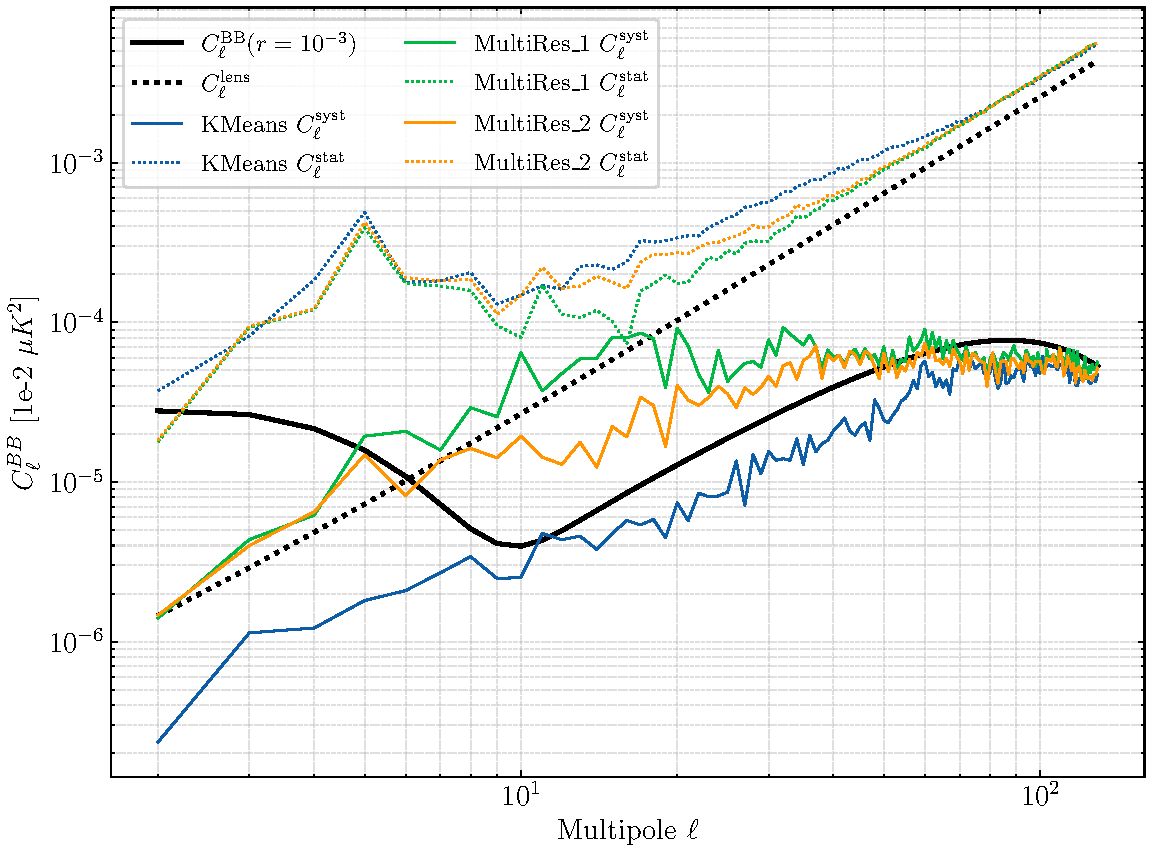
\includegraphics[width=\linewidth]{figures/bb_residual_spectra.pdf}
    \caption{
    Residual \( B \)-mode power spectra for single-patch, multi-resolution, and K-means clustering methods. 
    The MultiRes-1 case (\textit{cf.} Table~\ref{tab:multires_config}, Fig.~\ref{fig:multires_patches}) illustrates the limited adaptability of pixel downgrading: moving from \(N_{\mathrm{side}} = 4\) to \(N_{\mathrm{side}} = 8\) for example entails a large, discrete increase in patch count, preventing intermediate configurations. 
    This rigidity leads to overshooting, especially when increasing the patch granularity for \(T_d\) and \(\beta_s\) MultiRes-2 (Fig.\ref{tab:validation_config}).
    In contrast, K-means clustering (Fig.~\ref{fig:furax_patches}) enables fine-grained, data-driven tuning of spatial complexity, yielding lower residuals by balancing systematic leakage and statistical variance.\\
    \je{can you find more explicit naming? for KMeans MultiRes\_1/2 since this is the figure that people will take out of context when refering to your work ...)}\\
    \je{maybe "This work (optimal Kmeans technique)" or something like that ?  with a red color ? for KMeans}\\
    \je{figure Y label is DL BB and not CL BB and remove $1e-2$}
    }
    \label{fig:bb_spectra_comparison}
\end{figure*}

\subsection{Tensor-to-Scalar Ratio Estimation}
\label{subsec:r_estimation}

We now assess the impact of residual foreground contamination on the estimation of the tensor-to-scalar ratio \( r \).
For each spatial modeling strategy—K-means clustering, multi-resolution grouping, and single global patch—we compute the \( r \)-likelihood using the reconstructed \( B \)-mode power spectra.

Figure~\ref{fig:r_likelihood_distribution} shows the resulting normalized likelihood distributions aggregated over sky regions and noise realizations.

The K-means clustering approach yields the most accurate and precise measurement, with a likelihood distribution narrowly centered around the true \( r \) value. 
The multi-resolution method exhibits a slight positive bias and broader dispersion, consistent with increased statistical noise in the reconstruction. 
In contrast, the single-patch model produces a deceptively tight constraint but a significant bias, strongly overestimating \( r \) due to residual systematic contamination.
This behavior reflects the dominance of coherent residuals, which shift the likelihood peak while artificially reducing the inferred uncertainty.
These trends mirror those observed in the residual \( B \)-mode spectra and further demonstrate the importance of flexible spatial modeling to achieve unbiased and robust cosmological inference.

\paragraph{Summary of Results.}
\begin{itemize}
    \item \textbf{K-means clustering} achieves the tightest and most unbiased constraints on \( r \).
    \item \textbf{Multi-resolution grouping} shows slight bias and wider uncertainty due to statistical noise amplification. \je{this seems to contradict your earlier observation when you said that K-means was slightly noisier}
    \item \textbf{Single global patch} yields a biased estimate of \( r \) despite a narrow likelihood, driven by uncorrected systematic residuals.
\end{itemize}

\begin{figure*}
    \centering
    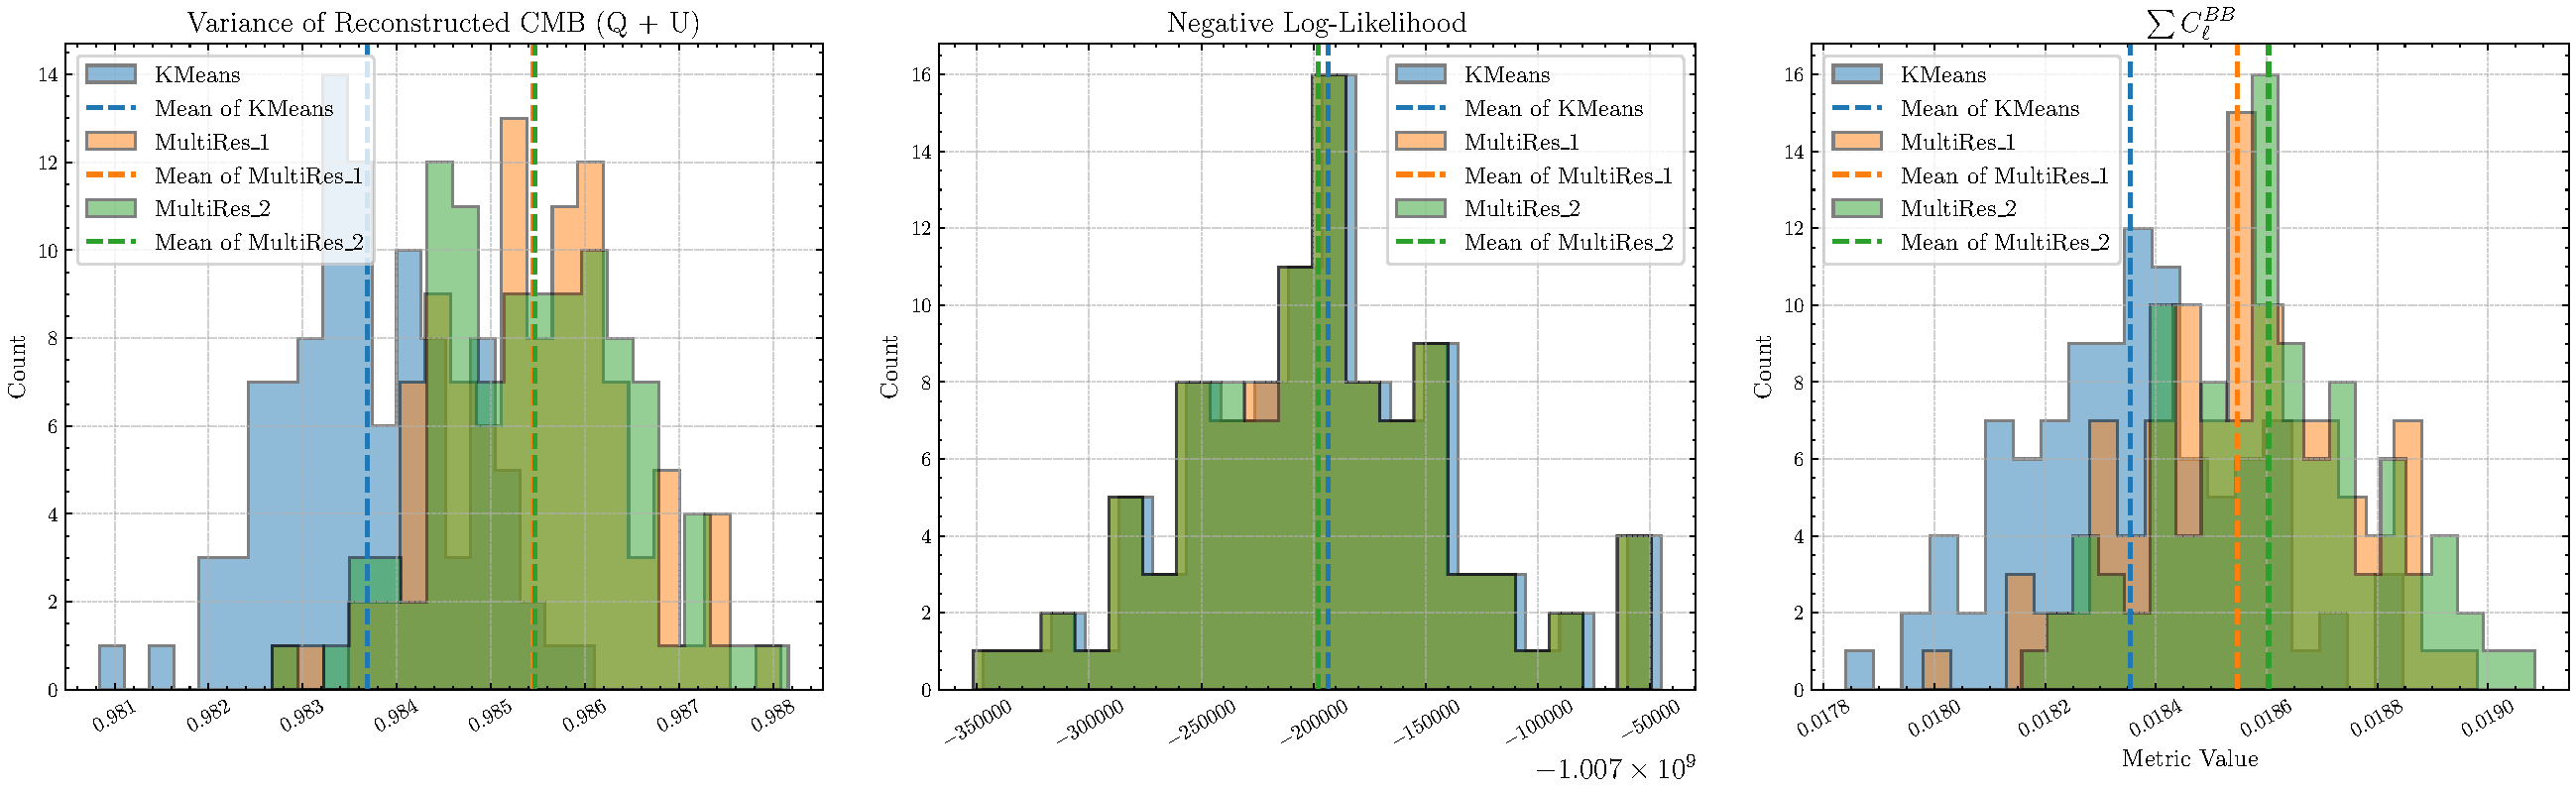
\includegraphics[width=1\linewidth]{figures/variance_likelihood_distributions.pdf}
    \caption{
    Distribution of evaluation metrics for three spatial modeling strategies: K-means clustering (see Fig.~\protect\ref{fig:furax_patches}), MultiRes-1 (Table~\protect\ref{tab:multires_config}, Fig.~\protect\ref{fig:multires_patches}), and MultiRes-2 (Table~\protect\ref{tab:validation_config}, shown in green). 
    Metrics shown are: W variance of the reconstructed CMB ($Q + U$), (center) negative log-likelihood, and (right) total $C_\ell^{BB}$ power. 
    Dashed vertical lines indicate the mean of each distribution. 
    K-means clustering yields the lowest residual variance and highest likelihood. 
    Multi-resolution approaches show broader distributions, reflecting higher statistical variability.
    }


    \label{fig:metric_distributions}
\end{figure*}

\vspace{-1em}

\begin{figure*}
    \centering
    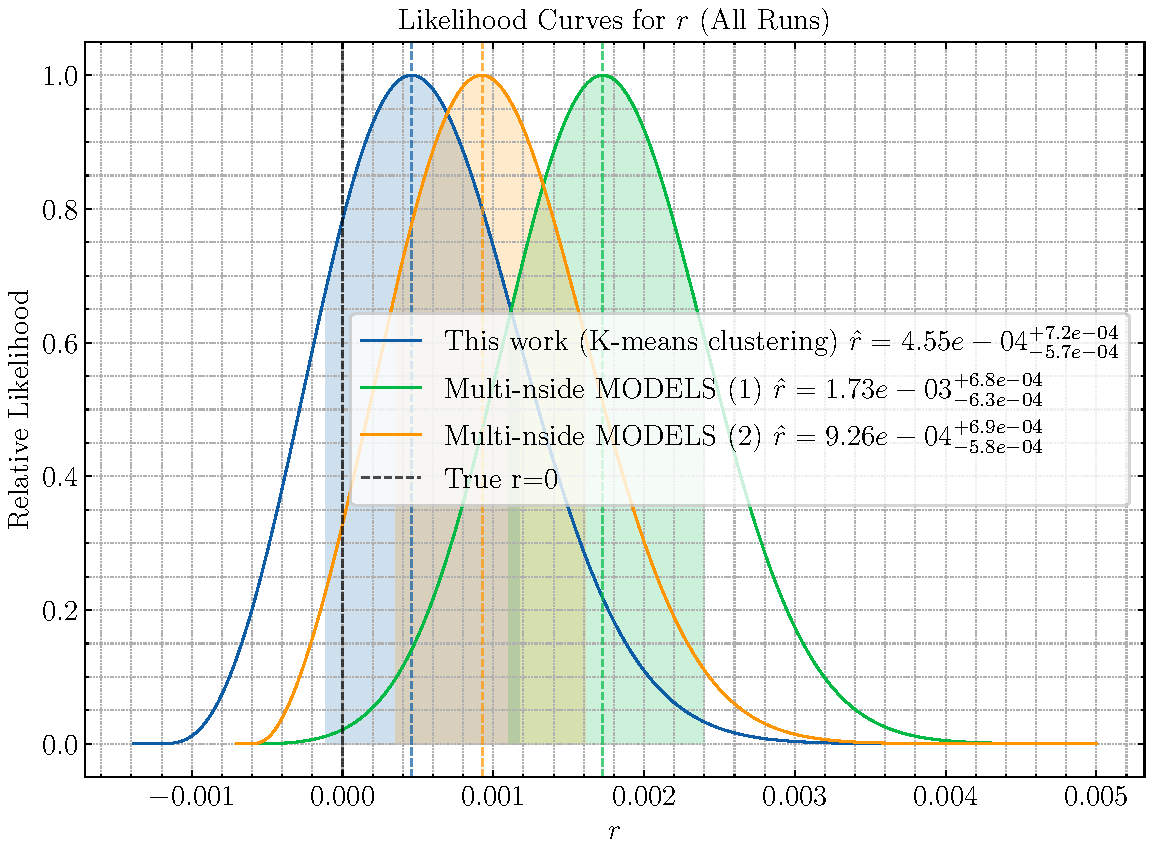
\includegraphics[width=0.9\linewidth]{figures/r_likelihood_distribution.pdf}
    \caption{
    \je{I don't think this figure was referred to nor commented  in the main text -- I think this is an important result!}
    Estimated tensor-to-scalar ratio likelihoods for K-means clustering (blue; see Fig.~\protect\ref{fig:furax_patches}), multi-resolution grouping with configurations MultiRes-1 (green; Table~\protect\ref{tab:multires_config}, Fig.~\protect\ref{fig:multires_patches}) and MultiRes-2 (orange; Table~\protect\ref{tab:validation_config}), compared to the true value \( r = 0 \). 
    K-means clustering yields the lowest bias (\( \hat{r} = 4.55 \times 10^{-4} \)) and tightest credible interval, while MultiRes-1 and MultiRes-2 exhibit increasing bias and broader uncertainty with finer granularity. 
    }
    
    \label{fig:r_likelihood_distribution}
\end{figure*}

\begin{figure*}
    \centering
    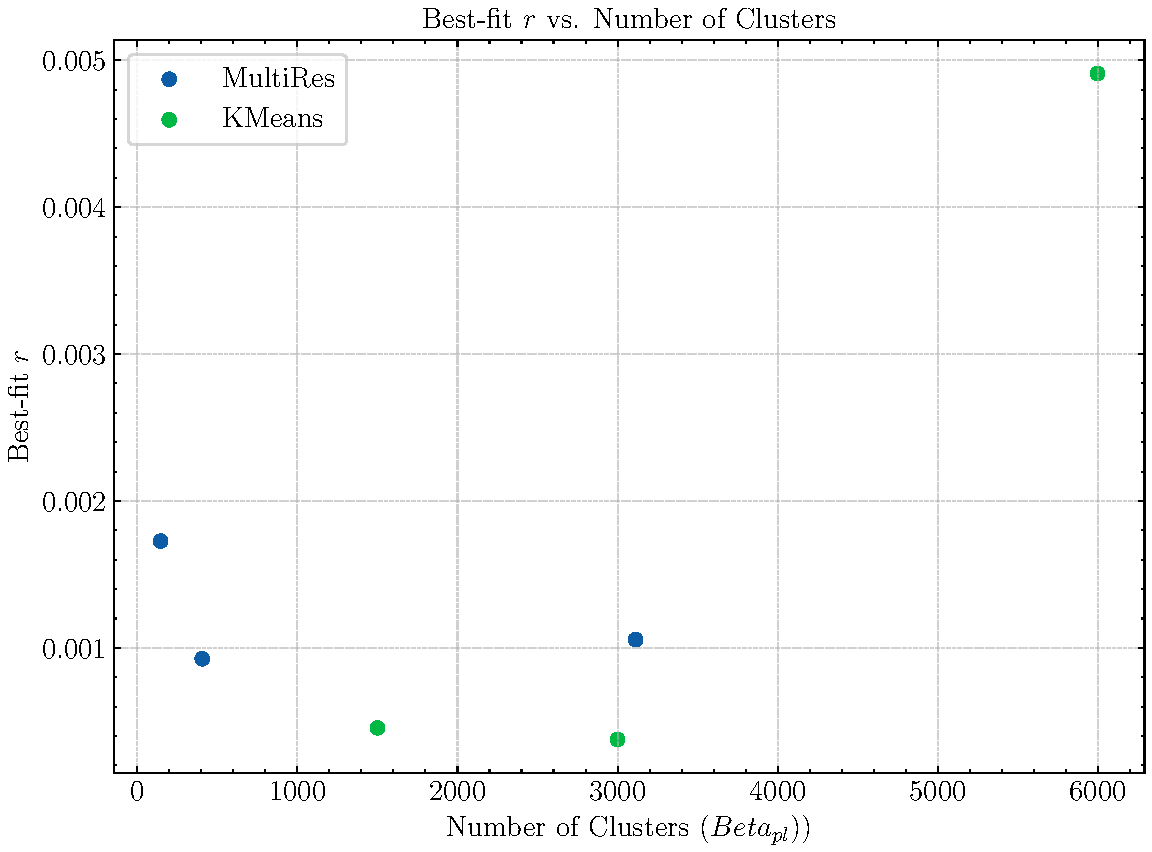
\includegraphics[width=0.9\linewidth]{figures/r_vs_clusters.pdf}
    \caption{
    Best-fit tensor-to-scalar ratio \( \hat{r} \) as a function of the number of clusters used for modeling the dust spectral index \( \beta_d \), comparing K-means clustering (green) and multi-resolution grouping (blue). 
    K-means supports finer-grained control over spatial complexity, enabling exploration of a broader and more continuous range of cluster counts. 
    In contrast, the multi-resolution approach is constrained by discrete HEALPix resolutions, resulting in coarser sampling and larger gaps between viable configurations.
    This flexibility allows K-means to achieve lower bias in \( \hat{r} \), particularly at intermediate clustering scales.
}    
    \label{fig:r_vs_clusters}
\end{figure*}


\subsection{Impact of Noise on Clustered Component Separation}
\label{subsec:noise_impact}

An important advantage of our approach lies in its adaptability to noise realization variability. In a multi-resolution approach, the spatial patch structure—defined by a fixed HEALPix downgrading—is predetermined and remains constant across noise realizations. This rigidity prevents the model from optimally dealing with noise-induced fluctuations in the data.

In contrast, our K-means clustering strategy combined with a grid search allows the patch configuration to be dynamically re-optimized for each noise realization. For any given realization, the clustering grid search evaluates multiple spatial partitionings and selects the one that minimizes the variance of the recovered CMB map. This flexibility enables the model to better mitigate noise-driven distortions in the spectral parameter estimates, particularly in low signal-to-noise regions.

As a result, the adaptive clustering approach can reduce residual foreground contamination and enhance the fidelity of component separation by effectively tailoring the patch structure to each specific noise scenario. This noise-aware reconfiguration leads to lower residual power and improves robustness in downstream cosmological inference.

\ar{\section{Towards lower statistical residuals}}


\je{C'est peut-être ici où Arianna pourrait insérer un nouveau paragraphe 5.8 
"post-clustering optimization" ?}

\section{Discussion}
\label{sec:discussion}

\je{careful with the repetitions with the conclusions ...} This work introduces a high-resolution, grid-based clustering approach for spatially varying parametric component separation, implemented in the modular and scalable \textsc{FURAX} \je{which shows important numerical improvement compared to previous implementations such as fgbuster} framework. Our objective was to evaluate whether learned \je{this sentence is not clear} spectral patch structures can offer advantages over fixed-resolution strategies, using an exhaustive scan over clustering configurations compared against a baseline multi-resolution method.

\subsection*{Foreground Modeling at Scale}

Rather than fixing patch scales by hand, as was done in~\citep{LiteBIRD_PTEP_2022}, we perform an exhaustive grid search over the number of patches per spectral parameter. This enables data-driven selection of spatial granularity, allowing each sky region to adopt the level of modeling complexity most appropriate to its foreground structure, as quantified by the variance in the recovered CMB map.

The resulting clusters, generated using spherical K-means, are highly flexible: patches are irregular, non-contiguous, and vary in size, adapting to the statistical structure of the input data. This avoids arbitrary binning and allows for more precise foreground modeling, particularly in regions with sharp spectral gradients or complex emission.

In contrast, the multi-resolution approach uses HEALPix downgrading to define fixed NSIDE patch maps. While fast and easy to implement, it lacks the capacity to adapt to regional sky complexity and yields higher residuals in zones with rapidly varying spectra. This difference highlights the value of learned patch structures in a data-driven way.

\je{here we'll be adding something about Arianna's further optimization}

\subsection*{Computational Scalability and Pipeline Design}

To support this large-scale scan---over 2 million component separation evaluations across 6 sky zones and 100 noise realizations per region---we leveraged distributed GPU parallelism using \texttt{jax-grid-search}. The entire sweep was completed in under 30 hours on 32 A100 GPUs across 4 nodes on the Jean Zay supercomputer.

Previous pipelines, including those used in~\cite{LiteBIRD_PTEP_2022}, could not scale to this volume: a single multi-patch likelihood fit could take up to 40 minutes, making exhaustive searches prohibitive. \texttt{FURAX} brings this class of analysis within reach, enabling principled exploration of spatial model structures at scale.

\subsection*{Reproducibility and Open Tools}

All results in this paper were produced using open-source software developed or co-developed by the author, including the \texttt{FURAX} framework and \texttt{jax-grid-search}. The full codebase used to generate the simulations, run the experiments, and produce the plots is publicly available at:

\begin{center}
\texttt{\href{https://github.com/ASKabalan/furax-compsep-paper}{https://github.com/ASKabalan/furax-compsep-paper}}
\end{center}

This ensures transparent and reproducible research, allowing others to easily re-run, extend, or adapt the pipeline for future use cases.

\subsection*{Limitations and Future Work}

While effective, our current strategy is based on a brute-force grid scan. This could be made more efficient using modern hyperparameter optimization techniques such as Tree-structured Parzen Estimators or Bayesian search.

Other directions for future work include:
\begin{itemize}
    \item Scaling to higher resolutions (e.g., \( N_{\text{side}} = 128 \) or \( 256 \))
    \item Adding priors on patch structure (e.g., smoothness or contiguity) \je{coming from e.g. external data sets}
    \item Exploring disjoint and irregular clustering with parameter sharing \je{that's now touched with Arianna's approach}
    \item Integrating additional systematic effects such as beam asymmetries, gain drift, or correlated noise
    \item Investigating alternative spatial modeling strategies beyond K-means, such as adaptive averaging of spectrally similar patches \je{touched by Arianna now. But we could mention that we may want to explore different shapes of masks for instance}
\end{itemize}


These extensions are naturally supported by the modular \texttt{FURAX} architecture and will be investigated in future work.

\subsection*{Limitations of Variance-Based Selection Criteria}

Although the variance of the reconstructed CMB and the total $\sum C_\ell^{BB}$ power are effective proxies for assessing residual contamination in the output CMB maps, \je{BEGIN : not sure what you mean here. Sum(ClBB) is sensitive to residuals in general -- not more statistical than systematics} these metrics can be sensitive to statistical residuals. As a result, they may sometimes overlook systematic residuals. \je{END}

In our analysis, we observed that relying solely on variance-based selection occasionally favored configurations with slightly elevated systematic residuals. \je{a better way to address this would be to fit for r directly! and the loss function would be given by r + sigma(r) for instance.  In that case, no need to adjust results by hand} To address this, we performed an additional manual inspection step: among the top-ranked configurations (with lowest variance), we selected the one that also satisfied a strict threshold on systematic residuals. This refinement ensures robust foreground cleaning and is reflected in the results shown in Figures~\ref{fig:metric_distributions}, \ref{fig:bb_spectra_comparison}, and \ref{fig:r_likelihood_distribution}.



\subsection*{Advanced Search Strategies for Cluster Configuration}

The choice of cluster configuration in our framework is better understood as part of a model selection problem, rather than a standard parameter estimation task. It determines the structure of the likelihood model itself—how spectral parameters are spatially grouped and constrained.

We experimented with more advanced search techniques to optimize cluster configuration, including the \texttt{Optuna}~\citep{OPTUNA} framework and discrete sampling strategies like Gibbs sampling. However, these methods showed limited improvements over exhaustive scanning, likely due to the discrete and highly non-smooth nature of the objective landscape.

Future efforts could explore:
\begin{itemize}
    \item Structured search methods that exploit correlations across sky zones
    \item Relaxed parameterizations that allow for differentiable optimization
\end{itemize}

For this work, the grid-based distributed search provided a robust and parallelizable solution, allowing exhaustive exploration of the model space in a tractable amount of time.

\section{Conclusions}
\label{sec:conclusion}

This work presents a new implementation of the parametric component separation approach, based on \texttt{JAX}. The new environment, called \texttt{FURAX} provides a modular environment to generalize the formalism to more complex data models, easing the explicit inclusion of e.g. instrumental response. Compared to previous implementation of similar ideas, for example \texttt{fgbuster}, we show that the new implementation is typically a factor X faster on CPUs and a factor Y faster on GPUs. 

In addition, the new implementation offers a scalable, flexible framework for a spatially varying characterization of CMB foregrounds, demonstrating the advantages of data-driven spectral patch selection through exhaustive clustering scans.

Compared to fixed-resolution baselines which were previously fine-tuned by hand, looking directly at the (in principle inaccessible) residuals, our approach yields:
\begin{itemize}
    \item Lower residual contamination in the reconstructed CMB maps
    \item Reduced bias and tighter constraints on the tensor-to-scalar ratio \( r \)
    \item Greater adaptability to complex Galactic foreground structures
\end{itemize}

By optimizing spectral patching using a physical criterion---the variance of the recovered CMB---we show that adaptive clustering improves both reconstruction fidelity and cosmological parameter estimation. 

The \texttt{FURAX} framework, fully open-source and scalable to millions of likelihood evaluations, provides a reproducible foundation for future high-fidelity CMB experiments targeting primordial \( B \)-mode polarization.

\section*{Acknowledgements}


The authors would like to thank Tran Hoang Viet, Arianna Rizzieri, Cl\'ement Leloup and Radek Stompor for useful exchanges during the development of this work. 

% The author would like to thank Josquin Errard for his guidance and supervision throughout this project. 
% Special thanks to Wuhyun Sohn for his extensive and thoughtful reviews, and to Benjamin Beringue for his valuable assistance with mathematical formulations.

This work was supported by the \textsc{SciPol} project (\href{https://scipol.in2p3.fr}{scipol.in2p3.fr}), funded by the European Research Council (ERC) under the European Union’s Horizon 2020 research and innovation program (Principal Investigator: Josquin Errard, Grant agreement No. 101044073). Some of the authors also benefited from the European Union’s Horizon 2020 research and innovation program under grant agreement no. 101007633 CMB-Inflate. 

The computations were performed using HPC resources provided by the \textit{Jean Zay} supercomputer at IDRIS under allocation 2024-AD010414161R2 granted by GENCI. 


% \section*{Acknowledgments}



% The \nocite command causes all entries in a bibliography to be printed out
% whether or not they are actually referenced in the text. This is appropriate
% for the sample file to show the different styles of references, but authors
% most likely will not want to use it.
% \nocite{*}
\bibliographystyle{mnras}
\bibliography{furax_comp_sep}% Produces the bibliography via BibTeX.

\end{document}
%
% ****** End of file apssamp.tex ******
